% Product Modification, Robinson-Patman, and Third-Degree Price Discrimination
\documentclass[12pt]{article}

% ── Packages ───────────────────────────────────────────────────────────────
\usepackage[margin=1in]{geometry}
\usepackage{amsmath,amssymb,amsthm}
\usepackage{booktabs}
\usepackage[dvipsnames,svgnames]{xcolor}
\usepackage{graphicx}
\graphicspath{{../figures/}}
\usepackage{hyperref}
\usepackage{setspace}
\usepackage{caption}
\usepackage{subcaption}
\usepackage{enumitem}
\usepackage{textcomp}
\usepackage[T1]{fontenc}
\usepackage{mathptmx}        % Times New Roman for body + math
\usepackage{float}
\usepackage{fancyhdr}

\doublespacing

% ── Headers ───────────────────────────────────────────────────────────────
\pagestyle{fancy}
\fancyhf{}
\fancyhead[L]{\small\textit{Product Modification and Price Discrimination}}
\fancyhead[R]{\small\thepage}
\setlength{\headheight}{14pt}
\renewcommand{\headrulewidth}{0pt}

% ── Theorem environments ──────────────────────────────────────────────────
\newtheorem{proposition}{Proposition}
\newtheorem{corollary}{Corollary}
\theoremstyle{definition}
\newtheorem{definition}{Definition}

% ── Hyperref ──────────────────────────────────────────────────────────────
\hypersetup{
    colorlinks=true,
    linkcolor=blue!70!black,
    citecolor=blue!70!black,
    urlcolor=blue!70!black,
}

\begin{document}

% ── Title Page ─────────────────────────────────────────────────────────────
\begin{titlepage}
\centering
\vspace*{2cm}
{\LARGE Product Modification, Robinson--Patman, and\\[6pt]
Third-Degree Price Discrimination\par}
\vspace{1.8cm}
\begin{tabular}{cc}
\textbf{Sophia Ng} & \textbf{Sohail (Neel) Sarkar} \\[4pt]
University of Toronto & University of Toronto \\
Department of Economics & Department of Mathematics \\
Honours BSc, Mathematics \& Economics & Honours BSc, Mathematics and its Applications \\[6pt]
\texttt{sophia.ng@mail.utoronto.ca} & \texttt{sohail.sarkar@mail.utoronto.ca}
\end{tabular}
\vspace{1.4cm}
{\large March 2026\par}
\vfill
\textit{Word count: approximately 9,500 (excluding tables, figures, and references)}
\end{titlepage}

% ABSTRACT
\newpage
\pagenumbering{roman}
\setcounter{page}{1}

\begin{abstract}
\noindent
This paper studies how minor product modifications in package size, formulation, or branding allow manufacturers to practice retailer-level third-degree price discrimination under the constraints of the Robinson--Patman Act (RPA).
A manufacturer--retailer model shows that introducing low-cost product variants outside the ``like grade and quality'' category relaxes a common-wholesale-price constraint and restores segment-specific pricing.
The model yields closed-form conditions under which product modification strictly increases manufacturer profit. It also characterizes a threshold differentiation cost $\bar{k}$ and expected legal penalty $L$ that together govern the choice between uniform pricing and variant-based discrimination.
The paper provides descriptive evidence consistent with two predictions using the Dominick's Finer Foods scanner dataset, which contains 3.24~million store-week-UPC observations spanning 566~laundry-detergent products across 93~stores and 396~weeks.
Regressions of per-unit price on log package size yield a coefficient of $-3.00$ (SE~$= 0.37$, $p < 0.001$), showing that larger packages carry significantly lower per-unit prices. This pattern is consistent with size-based surplus extraction.
Store fixed effects are jointly significant ($F = 15.04$, $p < 0.001$), documenting systematic cross-location pricing variation even within a single retail chain.
Brand fixed effects raise the $R^2$ from 0.38 to 0.47, indicating that brand-level product differentiation is a material channel for price discrimination.
The findings highlight how legal constraints, product design, and nonlinear pricing interact. They contribute to the law-and-economics discussion of Robinson--Patman and to the broader literature on third-degree price discrimination.
\end{abstract}

\medskip
\noindent
\textbf{Keywords:} price discrimination, Robinson--Patman Act, product differentiation, package size, scanner data, nonlinear pricing

\noindent
\textbf{JEL Codes:} L11, L42, K21, D42

\newpage
\tableofcontents
\newpage
\pagenumbering{arabic}
\setcounter{page}{1}

% INTRODUCTION
\section{Introduction}\label{sec:intro}

Firms with market power routinely charge different prices for similar products across customers, channels, or regions.
Standard industrial-organization theory treats this as third-degree price discrimination. The standard assumption is that the monopolist can freely set segment-specific prices as long as arbitrage is prevented.\footnote{A.~C. Pigou, \textit{The Economics of Welfare} (London: Macmillan, 1920); Hal~R. Varian, ``Price Discrimination,'' in \textit{Handbook of Industrial Organization}, vol.~1, ed.\ R.~Schmalensee and R.~Willig (Amsterdam: North-Holland, 1989), 597--654.}
In practice, however, price discrimination at the wholesale level in the United States is constrained by the Robinson--Patman Act (RPA). The RPA prohibits charging competing buyers different prices for commodities of ``like grade and quality'' when such discrimination may lessen competition.\footnote{Federal Trade Commission, ``Price Discrimination: Robinson-Patman Violations,'' \url{https://www.ftc.gov/advice-guidance/competition-guidance/guide-antitrust-laws/price-discrimination-robinson-patman-violations}, accessed March 2026.}

Manufacturers have responded by developing product and packaging strategies that maintain nominal compliance with the statute while achieving the same economic objectives as unconstrained price discrimination.
By creating retailer-specific package sizes, variant formulations, or cosmetic changes that generate distinct stock-keeping units (SKUs), firms can argue that goods are not of like grade and quality and therefore fall outside the statute's reach.
Recent case law, including the Seventh Circuit's decision in \textit{Woodman's Food Market v.\ Clorox}, confirms that the boundary between ``like'' and ``different'' commodities is central to assessing price differences across channels.\footnote{\textit{Woodman's Food Market, Inc.\ v.\ Clorox Co.}, No.\ 15-3001 (7th Cir.\ 2016).}

This paper asks:
\begin{quote}
\textit{How do minor product modifications enable manufacturers to implement retailer-level third-degree price discrimination under Robinson--Patman constraints, and what are the resulting implications for prices and welfare?}
\end{quote}

The analysis proceeds in three steps.
First, it develops a manufacturer--retailer model in which Robinson--Patman--type constraints impose a common wholesale price for identical products. The manufacturer can relax this constraint by introducing low-cost product variants.
Second, it links the model to actual legal institutions. It reviews FTC guidance and key case law to map specific product modifications into the legal framework.
Third, it provides descriptive evidence consistent with two predictions using the Dominick's Finer Foods scanner dataset: (i)~per-unit prices decrease with package size, consistent with size-based price discrimination, and (ii)~per-unit prices vary systematically across stores, consistent with heterogeneous local pricing conditions within the chain.

The contribution is twofold.
On the theory side, the paper formalizes a channel-specific price-discrimination mechanism that is widely discussed in legal practice but has received limited formal treatment.
On the empirical side, it provides a rigorous analysis of over 3.24~million scanner observations documenting pricing patterns consistent with the model: a steep size--price gradient, significant cross-store dispersion, and brand-level heterogeneity in per-unit pricing.

Section~\ref{sec:background} reviews the institutional and legal background.
Section~\ref{sec:literature} situates the analysis in the relevant literature.
Section~\ref{sec:model} presents the model and derives closed-form results.
Section~\ref{sec:empirical} describes the data and reports empirical findings.
Section~\ref{sec:cases} revisits case studies.
Section~\ref{sec:welfare} discusses welfare implications.
Section~\ref{sec:conclusion} concludes.
Appendix~\ref{app:welfare} provides a formal welfare comparison, Appendix~\ref{app:robustness} considers asymmetric markups, and Appendix~\ref{app:simulations} collects simulation figures.


% INSTITUTIONAL AND LEGAL BACKGROUND
\section{Institutional and Legal Background}\label{sec:background}

\subsection{The Robinson--Patman Act and ``like grade and quality''}

The Robinson--Patman Act, enacted in 1936, amended the Clayton Act to address perceived abuses in price discrimination by large suppliers against small retailers.\footnote{Federal Trade Commission, ``Price Discrimination: Robinson-Patman Violations,'' accessed March 2026.}
Section~2(a) prohibits charging different prices to competing purchasers for commodities of ``like grade and quality'' where the effect may be to substantially lessen competition.
Sections~2(d) and 2(e) prohibit discriminatory payments or services related to promotional activities. Section~2(f) targets buyers who knowingly induce or receive discriminatory prices.\footnote{Federal Trade Commission, ``Price Discrimination: Robinson-Patman Violations,'' accessed March 2026.}

The FTC's guidance emphasizes that price differences are not automatically unlawful.
Sellers can justify different prices through cost savings in manufacture or delivery. They can also show that lower prices were offered in good faith to meet a competitor's equally low price.
However, when a seller offers more favorable terms to certain buyers but not others, Sections~2(d) and 2(e) may apply.

A central concept in applying Section~2(a) is whether the commodities sold to different buyers are of ``like grade and quality.''
Courts have generally interpreted this phrase to refer to the physical characteristics of the goods rather than their marketing or packaging.
The case law shows, however, that features such as package size, special packaging, or promotional content can be relevant when they create materially different competitive conditions across retailers.\footnote{Crowell \& Moring LLP, ``Do Different Size Packages Violate the Robinson Patman Act?'' Client Alert, March 2015; McGuireWoods LLP, ``June Antitrust Bulletin,'' June 2015.}
This ambiguity gives manufacturers an incentive to design product modifications that are plausibly outside the ``like grade and quality'' category while still serving the same consumer function.

\subsection{Package size, packaging, and large-format SKUs}

One common form of product modification involves offering different package sizes to different classes of trade.
Club stores such as Costco and Sam's Club often receive large, multi-unit packages. Traditional supermarkets and convenience stores stock smaller sizes.

A prominent test case is \textit{Woodman's Food Market, Inc.\ v.\ Clorox Co.}, in which a regional supermarket chain alleged that Clorox violated Section~2(e) by refusing to sell it the large-size packages available to warehouse clubs.\footnote{\textit{Woodman's Food Market, Inc.\ v.\ Clorox Co.}, No.\ 15-3001 (7th Cir.\ 2016).}
The Seventh Circuit held that package size, standing alone, is not a ``promotional service or facility'' within the meaning of Section~2(e).
The court left open, however, the possibility that price discrimination associated with package size could be challenged under Section~2(a).\footnote{Crowell \& Moring LLP, ``Woodman's v.\ Clorox: Does Size Matter? Not Always Under the Robinson-Patman Act,'' Client Alert, 2016.}

Beyond package size, manufacturers use channel-specific SKUs distinguished by packaging, labeling, or minor formulation changes.
Legal advisors note that creating retailer-exclusive SKUs with distinct UPC codes can help demonstrate that goods sold to different retailers are not of like grade and quality. This reduces Robinson--Patman exposure.\footnote{Crowell \& Moring, ``Do Different Size Packages Violate the Robinson Patman Act?''}
These strategies also raise consumer search costs and make direct comparison across retailers more difficult, sustaining different markups for ostensibly similar products.

\subsection{Enforcement cycles and current policy debate}

Robinson--Patman enforcement has oscillated between aggressive periods and decades of relative dormancy as antitrust policy shifted toward a consumer-welfare standard.\footnote{Bruce~H. Kobayashi and Timothy~J. Muris, ``Stop Making Sense: Reviving the Robinson-Patman Act and the Economics of Intermediate Price Discrimination,'' February 2026.}
Critics argue that strict enforcement protects inefficient small retailers at the expense of lower consumer prices. Supporters counter that unchecked discrimination by powerful manufacturers and retailers can harm long-run competition.\footnote{Institute for New Economic Thinking, ``Chicago School Economists Got it Wrong: Strong Antitrust Policy Boosts the Economy,'' 2018; Information Technology and Innovation Foundation, ``No, Reviving the Robinson-Patman Act Will Not Lead to More Competition,'' November 2024.}

Recent policy discussions suggest renewed interest in Robinson--Patman enforcement, particularly given rising concentration in retail and wholesale markets.\footnote{Winston \& Strawn LLP, ``Price Discrimination Claims Under the Resurging Robinson-Patman Act,'' \textit{Competition Corner}, 2023.}
This makes it important to understand how firms adapt their pricing and product strategies in response to the statute.


% RELATED LITERATURE
\section{Related Literature}\label{sec:literature}

\subsection{Price discrimination and nonlinear pricing}

The textbook treatment of third-degree price discrimination considers a monopolist that segments markets and sets separate prices $p_i$ in each segment, equating marginal revenue to a common marginal cost $c$.\footnote{Pigou, \textit{The Economics of Welfare}; Varian, ``Price Discrimination,'' 597--654.}
Under linear demand, this implies higher prices in less elastic segments. Whether total welfare rises or falls relative to uniform pricing depends on how total output changes.

Nonlinear pricing frameworks generalize this logic to settings where consumer types are private information and firms design pricing schedules to induce self-selection.
Wilson analyzes two-part tariffs, block tariffs, and other nonlinear schemes as mechanisms that approximate first-degree price discrimination under incentive-compatibility constraints.\footnote{Robert~B. Wilson, \textit{Nonlinear Pricing} (Oxford: Oxford University Press, 1993).}
In these models, legal or regulatory constraints enter as restrictions on the menu of feasible contracts.

Bundling and tying provide another route to surplus extraction.
Adams and Yellen show that bundling can increase profits when consumers' valuations are negatively correlated. McAfee, McMillan, and Whinston extend this logic to multi-product monopolists with more general value structures.\footnote{W.~J. Adams and J.~L. Yellen, ``Commodity Bundling and the Burden of Monopoly,'' \textit{Quarterly Journal of Economics} 90, no.~3 (1976): 475--498.}

\subsection{Law-and-economics analyses of Robinson--Patman}

Law-and-economics scholarship on Robinson--Patman has long debated whether the statute promotes or undermines competitive outcomes.
Early critiques argued that Robinson--Patman conflicts with the consumer-welfare standard and that its focus on protecting individual competitors can punish pro-competitive differential pricing.\footnote{Kobayashi and Muris, ``Stop Making Sense.''}
More recent commentary emphasizes that targeted discounts to powerful retailers can foreclose rivals and dampen upstream competition.\footnote{``Winners and Losers under the Robinson-Patman Act,'' CBS Working Paper No.\ 30.}

Within this literature, package-size differences and special packaging have played an important role.
Analyses of \textit{Woodman's} and related disputes show that producers can segment channels by offering retailer-specific package sizes, often paired with different per-unit wholesale prices.
Yonezawa, G\'{o}mez, and Richards (2020) find that wholesale prices diverge across retailers despite Robinson--Patman constraints, but do not model the product-modification mechanism through which firms implement this divergence. The present paper fills that gap.\footnote{Koichi Yonezawa, Miguel~I.\ G\'{o}mez, and Timothy~J.\ Richards, ``The Robinson--Patman Act and Vertical Relationships,'' \textit{American Journal of Agricultural Economics} 102, no.~1 (2020): 329--352, \url{https://doi.org/10.1093/ajae/aaz049}. Accessed March 2026.}
This paper contributes by providing a tractable model in which product modification is an explicit decision variable that interacts with Robinson--Patman constraints. It also documents retail pricing patterns consistent with the model using large-scale scanner data.


% MODEL
\section{Model}\label{sec:model}

\subsection{Setup}

Consider a single upstream manufacturer that supplies a homogeneous good to two downstream retailers, indexed by $i \in \{1,2\}$.
Retailer $i$ sells to final consumers at retail price $p_i$ and faces linear demand
\begin{equation}\label{eq:demand}
Q_i(p_i) = a_i - b_i\, p_i, \quad a_i, b_i > 0.
\end{equation}
Retailer~1 has less elastic demand than retailer~2, so $b_1 < b_2$.
The manufacturer has constant marginal cost~$c$ and no fixed costs. Downstream marginal costs are normalized to zero.

The timing is as follows.
First, the manufacturer chooses a wholesale pricing and product-design strategy.
Second, retailers observe their wholesale prices and apply fixed markups $m_i$, so $p_i = w_i + m_i$.
This fixed-markup assumption abstracts from strategic interaction between the manufacturer and retailers. It can be relaxed in extensions (see Appendix~\ref{app:robustness}).

A Robinson--Patman--type legal constraint applies when the manufacturer sells identical commodities to both retailers: the manufacturer must charge a common wholesale price $w$.
Differential pricing is allowed only if the products sold are not of ``like grade and quality.''
The manufacturer can, at per-unit cost $k \ge 0$, introduce two distinct product variants, $A$ and $B$, sold exclusively to retailers 1 and 2 respectively.

\subsection{Uniform-pricing benchmark}

Under uniform pricing, the manufacturer supplies an identical product at wholesale price $w$.
Retail prices are $p_i = w + m_i$, quantities are $Q_i(w) = a_i - b_i(w + m_i)$, and profit is
\begin{equation}\label{eq:pi_u_fn}
\Pi^U(w) = (w - c)\sum_{i=1}^{2}\bigl(a_i - b_i(w + m_i)\bigr).
\end{equation}
The first-order condition yields the profit-maximizing common wholesale price
\begin{equation}\label{eq:wstar}
w^* = \frac{\sum_{i} a_i - \sum_{i} b_i m_i + c\sum_{i} b_i}{2\sum_{i} b_i}.
\end{equation}
Substituting back, optimal uniform-pricing profit is
\begin{equation}\label{eq:pi_u}
\Pi^U = \frac{\Bigl(\sum_i (a_i - b_i m_i) - c\sum_i b_i\Bigr)^2}{4\sum_i b_i}.
\end{equation}

Figure~\ref{fig:profit_curve} plots $\Pi^U(w)$ as a function of the common wholesale price. The concave quadratic peaks at $w^*$. The dashed horizontal line marks the higher profit level $\Pi^D$ achievable once the RPA constraint is relaxed through product modification.

\begin{figure}[H]
\centering
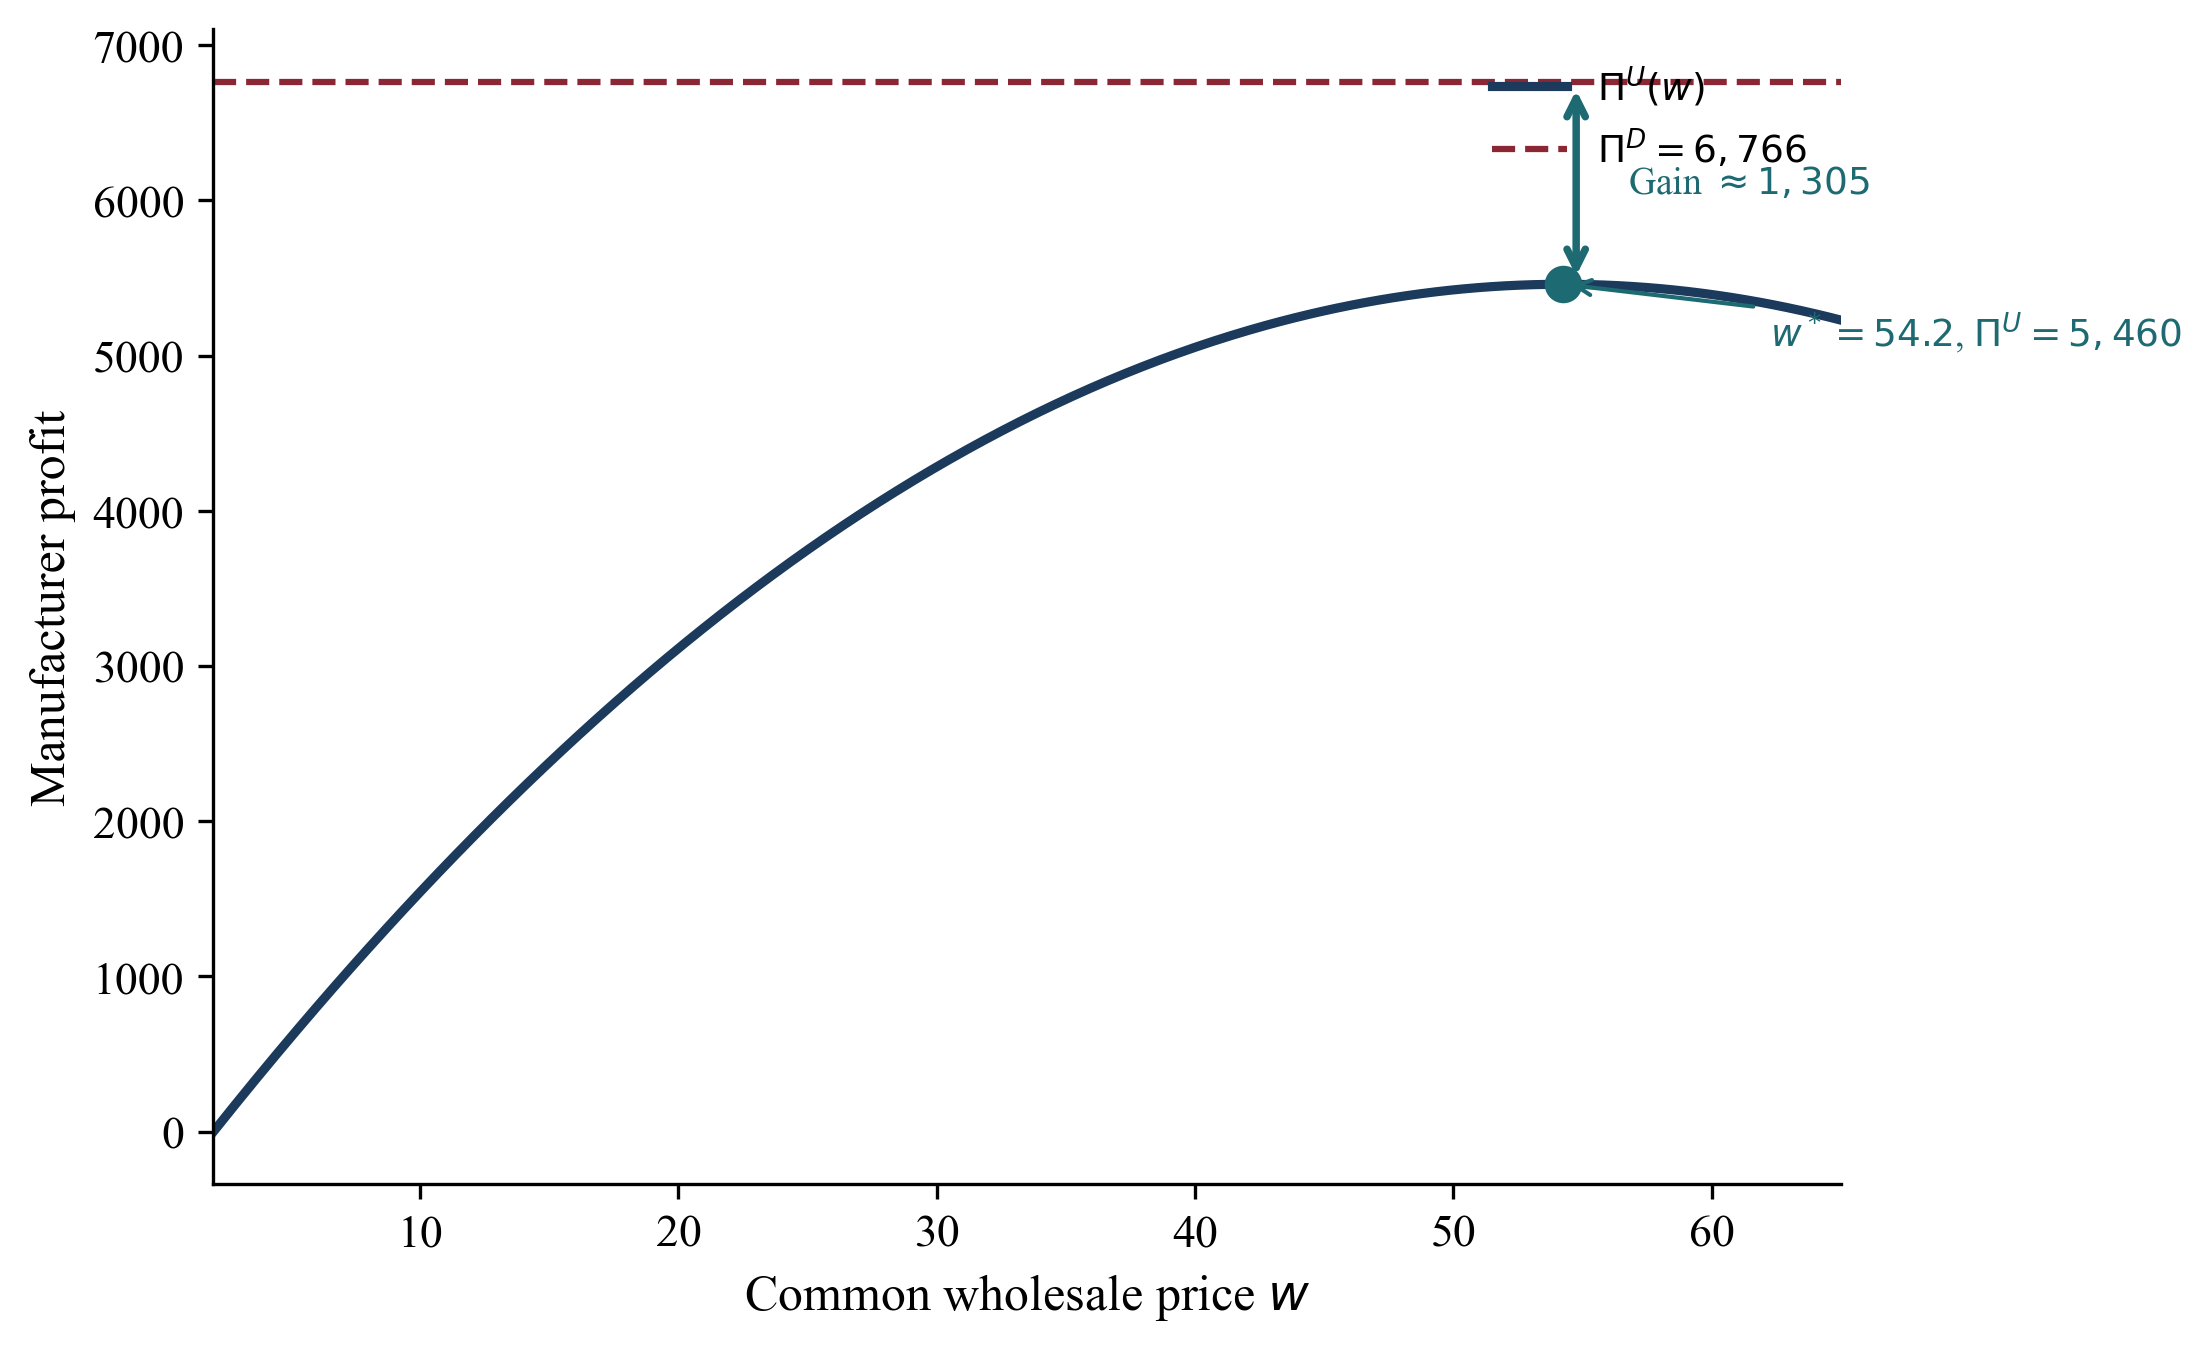
\includegraphics[width=0.82\textwidth]{fig1_profit_curve.png}
\caption{Manufacturer profit as a function of the common wholesale price $w$ under uniform pricing. The dashed line shows the discriminatory profit $\Pi^D$ when variants allow segment-specific pricing. The arrow marks the profit gain from Proposition~\ref{prop:profit}. \textit{Source:} Author's calculations based on model parameters.}
\label{fig:profit_curve}
\end{figure}

\subsection{Product modification and discriminatory wholesale pricing}

Suppose the manufacturer creates two variants at per-unit differentiation cost $k \ge 0$, charging $w_1$ for variant $A$ and $w_2$ for variant $B$.
Profit under discrimination is
\begin{equation}\label{eq:pi_d_fn}
\Pi^D(w_1,w_2;k) = \sum_{i=1}^{2}(w_i - c - k)\bigl(a_i - b_i(w_i + m_i)\bigr).
\end{equation}
Maximizing independently over each $w_i$ yields
\begin{equation}\label{eq:wi}
w_i^* = \frac{a_i - b_i m_i + b_i(c+k)}{2b_i} = \frac{a_i}{2b_i} - \frac{m_i}{2} + \frac{c+k}{2}.
\end{equation}
Two points follow.
First, without Robinson--Patman constraints, the manufacturer would choose these segment-specific prices even without product modification.
Second, when the law requires a common $w$ for identical products, product modification allows the manufacturer to implement $w_1^*$ and $w_2^*$ despite the constraint. This holds provided the variants are legally sufficient to escape the ``like grade and quality'' definition.

Optimal discriminatory profit has the closed form
\begin{equation}\label{eq:pi_d}
\Pi^D(k) = \sum_{i=1}^{2}\frac{\bigl(a_i - b_i m_i - b_i(c+k)\bigr)^2}{4b_i}.
\end{equation}
We assume throughout that $k$ is small enough that $Q_i^D > 0$ for each segment, i.e., $k < \hat{k}_i \equiv a_i/b_i - m_i - c$ for all $i$. This ensures both markets are profitably served at the discriminatory optimum, so the formulae above correctly characterise the manufacturer's equilibrium profit.

\subsection{Price elasticities and the Ramsey condition}

At the discriminatory equilibrium, the retail price in segment $i$ is $p_i^D = w_i^* + m_i$, and the quantity is $Q_i^D = a_i - b_i p_i^D$.
The price elasticity of demand in segment $i$ at this equilibrium is
\begin{equation}\label{eq:elasticity}
\varepsilon_i = -\,b_i\,\frac{p_i^D}{Q_i^D}.
\end{equation}
The optimal pricing rule satisfies the standard inverse-elasticity (Ramsey) condition:
\begin{equation}\label{eq:ramsey}
\frac{p_i^D - (c+k)}{p_i^D} = \frac{1}{|\varepsilon_i|}.
\end{equation}
The segment with higher $|\varepsilon_i|$ receives the lower markup. This connects the model directly to the classical third-degree discrimination result.\footnote{Varian, ``Price Discrimination,'' 601--605.}

\subsection{Profit comparison and threshold differentiation cost}

Let $\Pi^D(k)$ and $\Pi^U$ denote optimal profits under discrimination (equation~\ref{eq:pi_d}) and uniform pricing (equation~\ref{eq:pi_u}) respectively.
Differentiation is profitable whenever $\Pi^D(k) > \Pi^U$.
Since $\Pi^D(k)$ is strictly decreasing in $k$, there exists a threshold $\bar{k} > 0$ such that
\begin{equation}\label{eq:threshold}
\Pi^D(k) > \Pi^U \quad\Longleftrightarrow\quad k < \bar{k}.
\end{equation}

\begin{proposition}[Profit effect of product modification]\label{prop:profit}
Suppose demand is linear and downstream markups are fixed.
If $\frac{a_1 - b_1 m_1}{b_1} \ne \frac{a_2 - b_2 m_2}{b_2}$ and $k = L = 0$, then $\Pi^D(0) > \Pi^U$.
\end{proposition}

\begin{proof}
The uniform-pricing profit function $\Pi^U(w)$ is a concave quadratic in $w$ (equation~\ref{eq:pi_u_fn}).
Its unique maximum is at $w^*$ (equation~\ref{eq:wstar}).
Under discrimination with $k=0$, the manufacturer solves two independent concave problems. The solution sets $w_i^* = (a_i - b_im_i + b_ic)/(2b_i)$ for each $i$.

These two segment-specific optima coincide at a single $w$ if and only if
\[
\frac{a_1 - b_1 m_1 + b_1 c}{2b_1} = \frac{a_2 - b_2 m_2 + b_2 c}{2b_2},
\]
For all but a measure-zero set of demand parameters, $w_1^* \ne w_2^*$. Coincidence would require the knife-edge equality $(a_1 - b_1 m_1)/b_1 = (a_2 - b_2 m_2)/b_2$, which holds on a Lebesgue-measure-zero set of parameter values. Under the maintained assumption $b_1 \ne b_2$, the knife-edge condition generically fails, so $w_1^* \ne w_2^*$, and any common $w$ forces at least one segment away from its unconstrained optimum.

By the envelope theorem, the constrained maximum of a smooth objective is weakly less than the unconstrained maximum. The inequality is strict because the constraint $w_1 = w_2$ is binding when $b_1 \ne b_2$. Therefore $\Pi^D(0) > \Pi^U$.
\end{proof}

\paragraph{Remark.}
The condition in Proposition~\ref{prop:profit} holds generically. In particular, when $b_1 \ne b_2$, equality of the two ratios requires a knife-edge parameter restriction.

\begin{proposition}[Threshold differentiation cost and legal risk]\label{prop:threshold}
There exists $\bar{k} > 0$ such that, for sufficiently small expected legal penalty $L$, the manufacturer prefers variant-based discrimination if and only if $k < \bar{k}$.
Moreover, $\bar{k}$ is increasing in $|b_1 - b_2|$ and decreasing in $L$.
\end{proposition}

\begin{proof}
From equation~\eqref{eq:pi_d}, $\Pi^D(k)$ is continuous and strictly decreasing in $k$, with $\Pi^D(0) > \Pi^U$ by Proposition~\ref{prop:profit}.
As $k$ increases, the discriminatory quantities $Q_i^D(k) = (a_i - b_i m_i - b_i(c+k))/2$ decline monotonically, reaching zero at $\hat{k}_i = a_i/b_i - m_i - c$. Denoting $\bar{k}_{\max} = \min_i \hat{k}_i$ and restricting attention to the feasible region $k \in [0, \bar{k}_{\max})$, differentiating equation~\ref{eq:pi_d} gives $\partial \Pi^D/\partial k = -\sum_i (a_i - b_i m_i - b_i(c+k))/2 < 0$, so $\Pi^D(k)$ is strictly decreasing on this interval and approaches zero as $k \to \bar{k}_{\max}$.
By continuity and strict monotonicity of $\Pi^D$, there exists a unique $\bar{k} \in (0, \bar{k}_{\max})$ satisfying $\Pi^D(\bar{k}) = \Pi^U$.

For comparative statics, note that $\Pi^D(0) - \Pi^U$ is increasing in $|b_1 - b_2|$: greater demand heterogeneity makes the uniform-price compromise costlier. Since $\Pi^D(k)$ shifts down uniformly as $k$ rises, greater $|b_1 - b_2|$ raises the starting level of $\Pi^D$ and therefore raises $\bar{k}$.
When legal risk $L > 0$ enters additively (the manufacturer compares $\Pi^U$ with $\Pi^D(k) - L$), the effective break-even condition is $\Pi^D(\bar{k}) = \Pi^U + L$. This tightens the threshold: $\bar{k}$ decreases in $L$.
\end{proof}

\paragraph{Closed-form expression for $\bar{k}$.}
Setting $\Pi^D(\bar{k}) = \Pi^U + L$ and expanding, define
\[
S_i(k) \equiv a_i - b_i m_i - b_i(c+k),
\]
so that $\Pi^D(k) = \sum_i S_i(k)^2/(4b_i)$.
Let $\Sigma \equiv \sum_i b_i$, $A \equiv \sum_i(a_i - b_im_i)$, and $R \equiv A - c\Sigma$, so that $\Pi^U = R^2/(4\Sigma)$.
Then $\bar{k}$ solves
\begin{equation}\label{eq:kbar_solve}
\sum_{i=1}^{2}\frac{(S_i(0) - b_i\bar{k})^2}{4b_i} = \frac{R^2}{4\Sigma} + L.
\end{equation}
Expanding the left side and collecting terms in $\bar{k}$ gives a quadratic:
\begin{equation}\label{eq:kbar_quadratic}
\frac{\Sigma}{4}\,\bar{k}^2 - \frac{1}{2}\!\left(\sum_i S_i(0)\right)\bar{k} + \left[\sum_i \frac{S_i(0)^2}{4b_i} - \frac{R^2}{4\Sigma} - L\right] = 0.
\end{equation}
The economically relevant (positive, smaller) root gives the threshold.
In the symmetric-markup case ($m_1 = m_2 = m$), this simplifies further and can be solved in closed form by the quadratic formula.

Figure~\ref{fig:kL_frontier} plots the break-even boundary $\bar{k}(L)$ in $(k, L)$-space. The blue-shaded region represents parameter combinations under which variant-based discrimination is optimal. The red-shaded region indicates that uniform pricing dominates.

\begin{figure}[H]
\centering
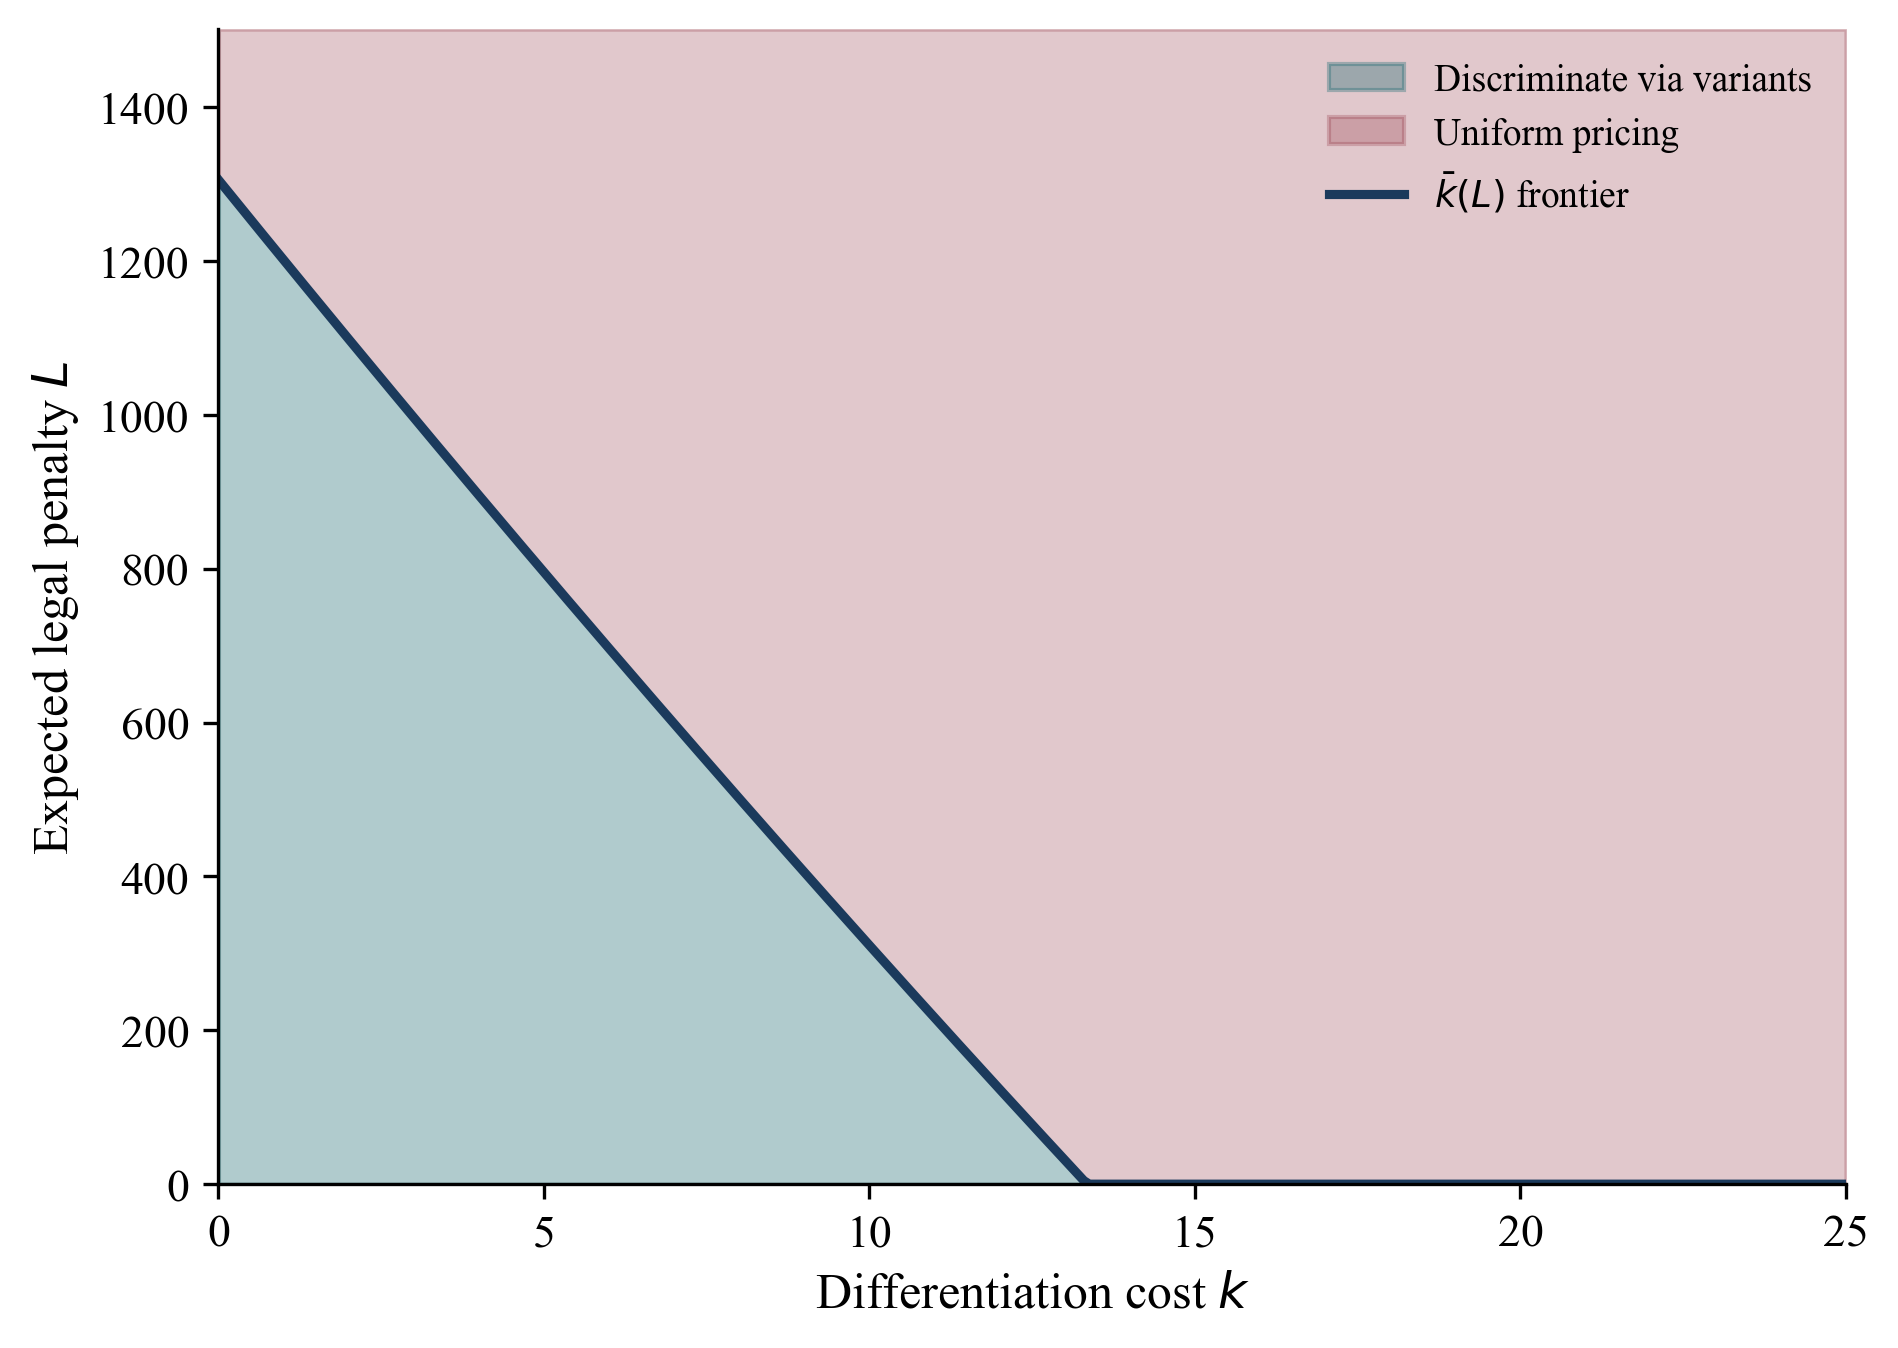
\includegraphics[width=0.82\textwidth]{fig4_kL_frontier.png}
\caption{Strategy frontier in $(k, L)$-space (Proposition~\ref{prop:threshold}). The curve traces the boundary $\bar{k}(L)$. Below the curve, the manufacturer profits from creating channel-specific variants. Above it, uniform pricing dominates. \textit{Source:} Author's calculations based on model parameters.}
\label{fig:kL_frontier}
\end{figure}


% EMPIRICAL ANALYSIS
\section{Descriptive Evidence from Dominick's Data}\label{sec:empirical}

\subsection{Data: Dominick's Finer Foods scanner dataset}

The empirical analysis uses the Dominick's Finer Foods scanner dataset, a widely studied panel of retail transactions from a major Chicago-area supermarket chain.\footnote{Dominick's Finer Foods Dataset, James~M.\ Kilts Center for Marketing, University of Chicago Booth School of Business, \url{https://www.chicagobooth.edu/research/kilts/research-data/dominicks}.}
The dataset contains two files: a UPC-level product lookup table (582~products) with product descriptions, package sizes, and case-pack counts, and a store-week-UPC movement file (approximately 6.74~million observations) recording shelf prices, unit sales, promotional indicators, and store identifiers.

The analysis focuses on the laundry-detergent category.
The raw product lookup contains package-size information as text strings with mixed units (for example, ``290~OZ,'' ``25~LB,'' ``150~EA'').
Sizes were parsed and converted to a common unit (fluid ounces), with pounds converted at $1~\text{lb} = 16~\text{oz}$.
Products denominated in non-convertible units (such as loads or count) were excluded, retaining 569 of 582~UPCs.
The lookup table was merged with the movement file on UPC.

Three filters were applied.
First, observations with zero shelf price or zero unit movement were dropped. These represent weeks in which a product was stocked but not sold.
Second, observations flagged as data-quality failures ($\texttt{OK} \ne 1$) were removed.
Third, per-unit prices in the top and bottom 0.1\% of the distribution were trimmed to limit the influence of likely data errors.
For multi-unit deals ($\texttt{QTY} > 1$), the effective unit price was computed as $\texttt{PRICE}/\texttt{QTY}$.

The final sample contains \textbf{3,240,409} store-week-UPC observations across \textbf{566~UPCs}, \textbf{93~stores}, and \textbf{396~weeks}.
Brands were extracted from product descriptions using string matching against known brand names (Tide, All, Wisk, Surf, Cheer, Era, Purex, and others).
A binary sale indicator equals one when the promotional flag is non-missing.

Khan and Jain (2005) document a steep size--price gradient in the same Dominick's dataset using over-the-counter painkiller products, consistent with second-degree price discrimination.\footnote{Romana~J.\ Khan and Dipak~C.\ Jain, ``An Empirical Analysis of Price Discrimination Mechanisms and Retailer Profitability,'' \textit{Journal of Marketing Research} 42, no.~4 (2005): 516--524.} The present paper extends this to third-degree discrimination across retail channels and connects the pricing pattern to Robinson--Patman compliance strategy.

\subsection{Variable construction}

The dependent variable is per-unit price:
\begin{equation}\label{eq:ppu}
\text{ppu}_{ijt} = \frac{\text{Price}_{ijt}\,/\,\text{QTY}_{ijt}}{\text{Size}_i} \times 100,
\end{equation}
expressed in cents per ounce, where $i$ indexes products (UPCs), $j$ indexes stores, and $t$ indexes weeks.
The primary independent variable is $\ln(\text{Size}_i)$, the natural logarithm of package size in ounces.
Additional controls include store fixed effects (93 store dummies), brand fixed effects (23 brand dummies), and the sale indicator.

\subsection{Descriptive statistics}

Table~\ref{tab:summary} reports summary statistics.
The average posted shelf price is \$5.57 (SD~\$3.19). The average package size is 87~oz (SD~55~oz). The average per-unit price is 7.21~\textcent/oz (SD~3.10).
Package sizes range from 2~oz single-use packets to 400~oz bulk containers. This generates substantial within-category variation in the size--price schedule.

\begin{table}[htbp]
\centering
\caption{Summary Statistics: Dominick's Laundry Detergent Scanner Data}
\label{tab:summary}
\small
\begin{tabular}{l rrrr rrrr}
\toprule
 & $N$ & Mean & SD & Min & P25 & Median & P75 & Max \\
\midrule
Price (\$) & 3,240,409 & 5.57 & 3.19 & 0.15 & 3.29 & 4.79 & 6.89 & 24.49 \\
Size (oz) & 3,240,409 & 87.24 & 54.92 & 2.00 & 50.00 & 70.00 & 110.00 & 400.00 \\
Per-unit price (\textcent/oz) & 3,240,409 & 7.21 & 3.10 & 2.25 & 5.21 & 6.86 & 8.34 & 60.36 \\
\bottomrule
\end{tabular}

\medskip\par\noindent\footnotesize
\textit{Notes:} Dominick's Finer Foods scanner data, laundry detergent category. Sample restricted to store-week-UPC observations with positive price, positive unit movement, and ounce-convertible package sizes. $N = 3,240,409$ observations across 93 stores, 566 UPCs, and 396 weeks.
\end{table}


\subsection{Descriptive figures}

Figure~\ref{fig:scatter} plots per-unit price against package size on a log-scaled horizontal axis, with observations colored by brand.
The negative log-linear relationship is visually clear: larger packages carry sharply lower per-unit prices.
The log-linear fit yields a slope of approximately $-3.0$. A doubling of package size is associated with roughly a 2.1~\textcent/oz decrease in per-unit price.
Brand-level clustering is also visible. Tide products, for instance, tend to occupy a higher price tier than Surf or Purex at comparable sizes.

\begin{figure}[H]
\centering
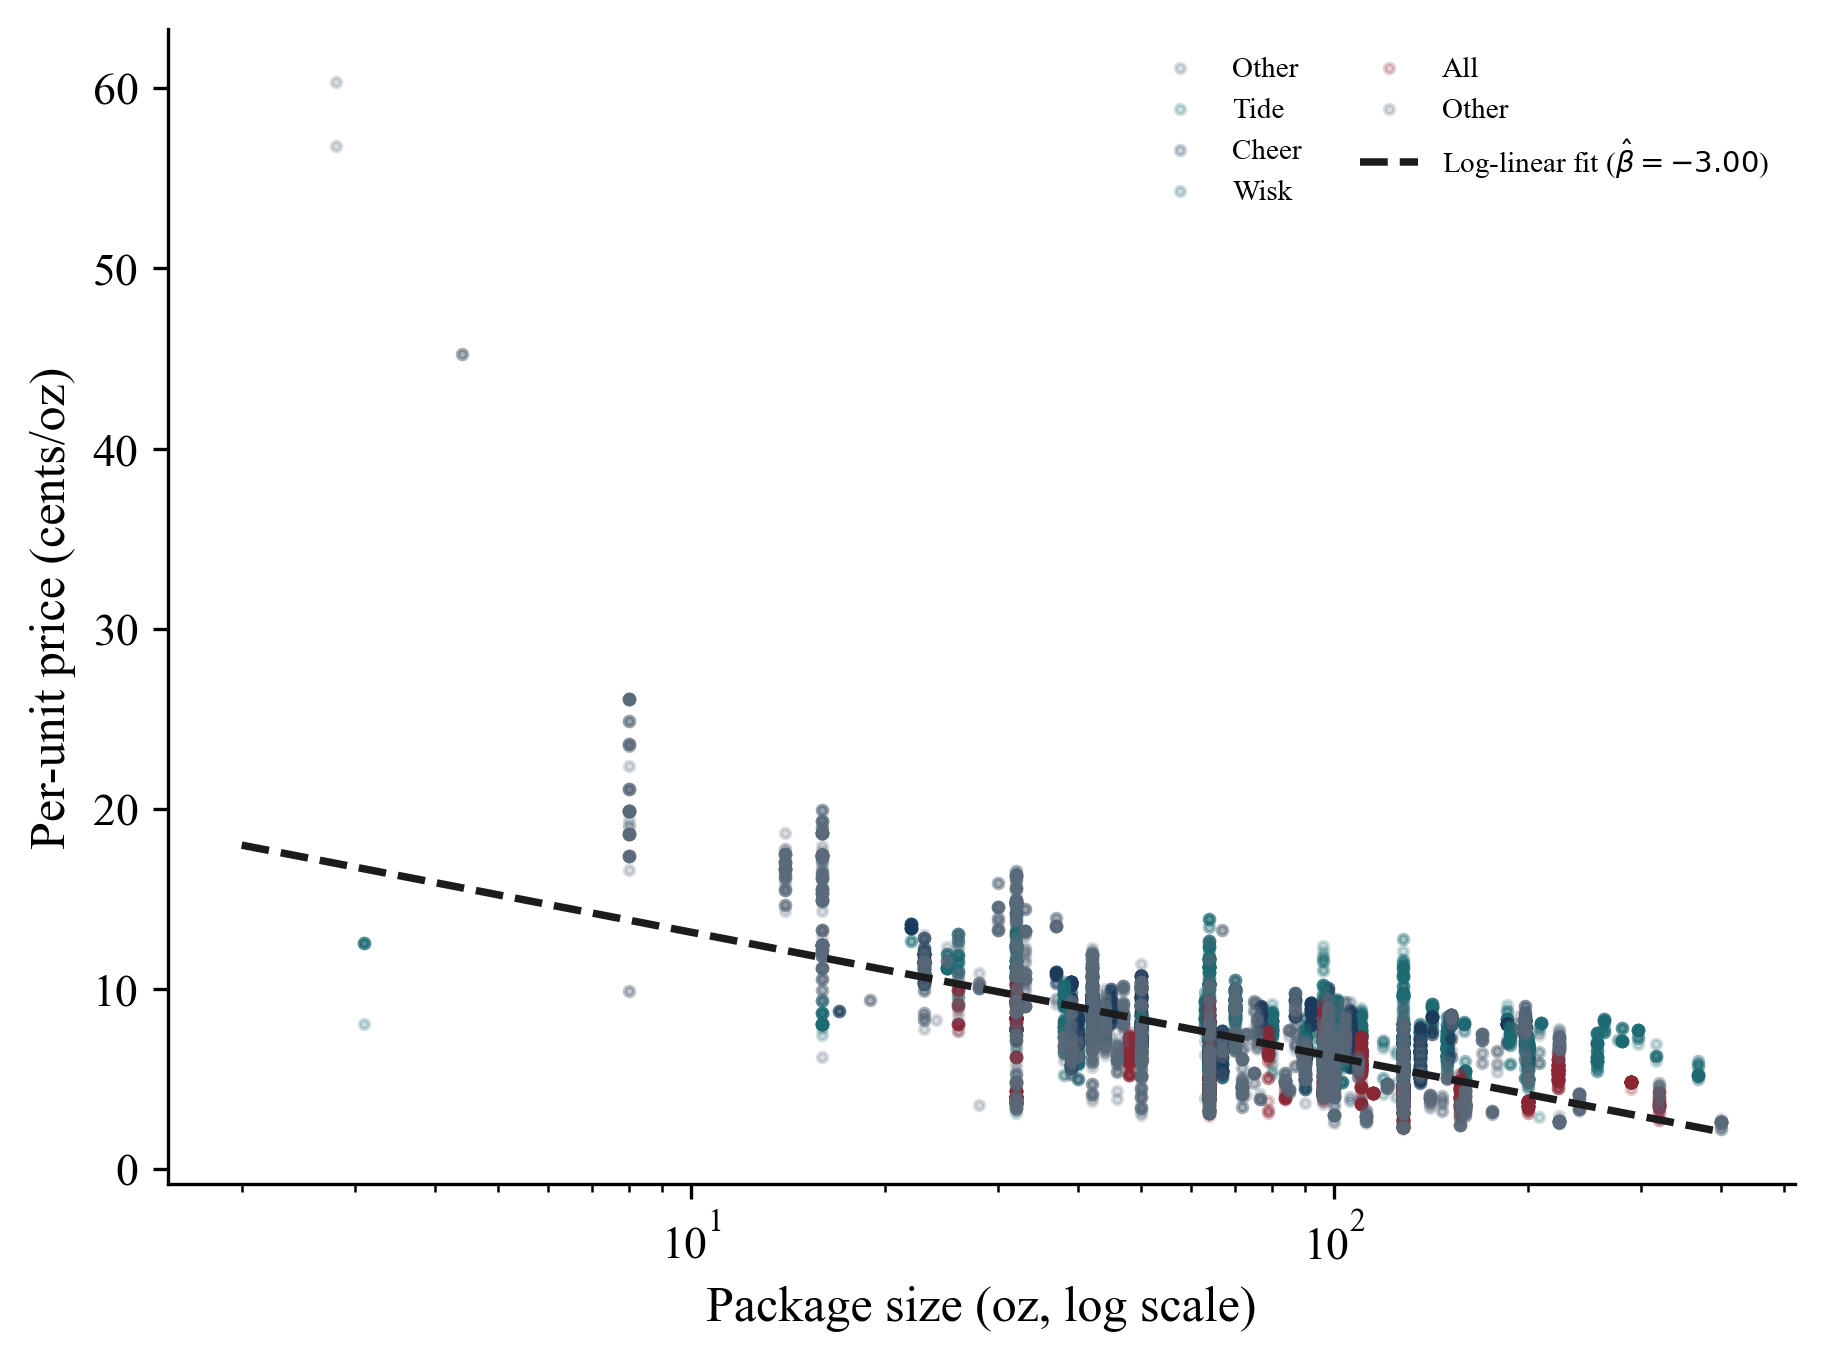
\includegraphics[width=0.82\textwidth]{fig6_size_vs_ppu.png}
\caption{Package size and per-unit price (laundry detergent, Dominick's data). Each point is a store-week-UPC observation. Colors indicate the five most common brands. The dashed line shows the log-linear fit. \textit{Source:} Author's calculations from Dominick's scanner data.}
\label{fig:scatter}
\end{figure}

Figure~\ref{fig:scatter_channel} presents the same scatter but distinguishes standard SKUs from large-format SKUs. Products in the largest 5\% of package sizes are marked separately (square markers); this top-5\% threshold is a proxy, since the Dominick's data cover a single supermarket chain and true channel-exclusive SKUs are not labelled directly. These bulk-size packages cluster in the bottom-right of the figure: low per-unit prices and large sizes. This pattern is consistent with the model's prediction that size-based product modification allows manufacturers to serve more elastic, bulk-buying segments at lower per-unit prices.

\begin{figure}[H]
\centering
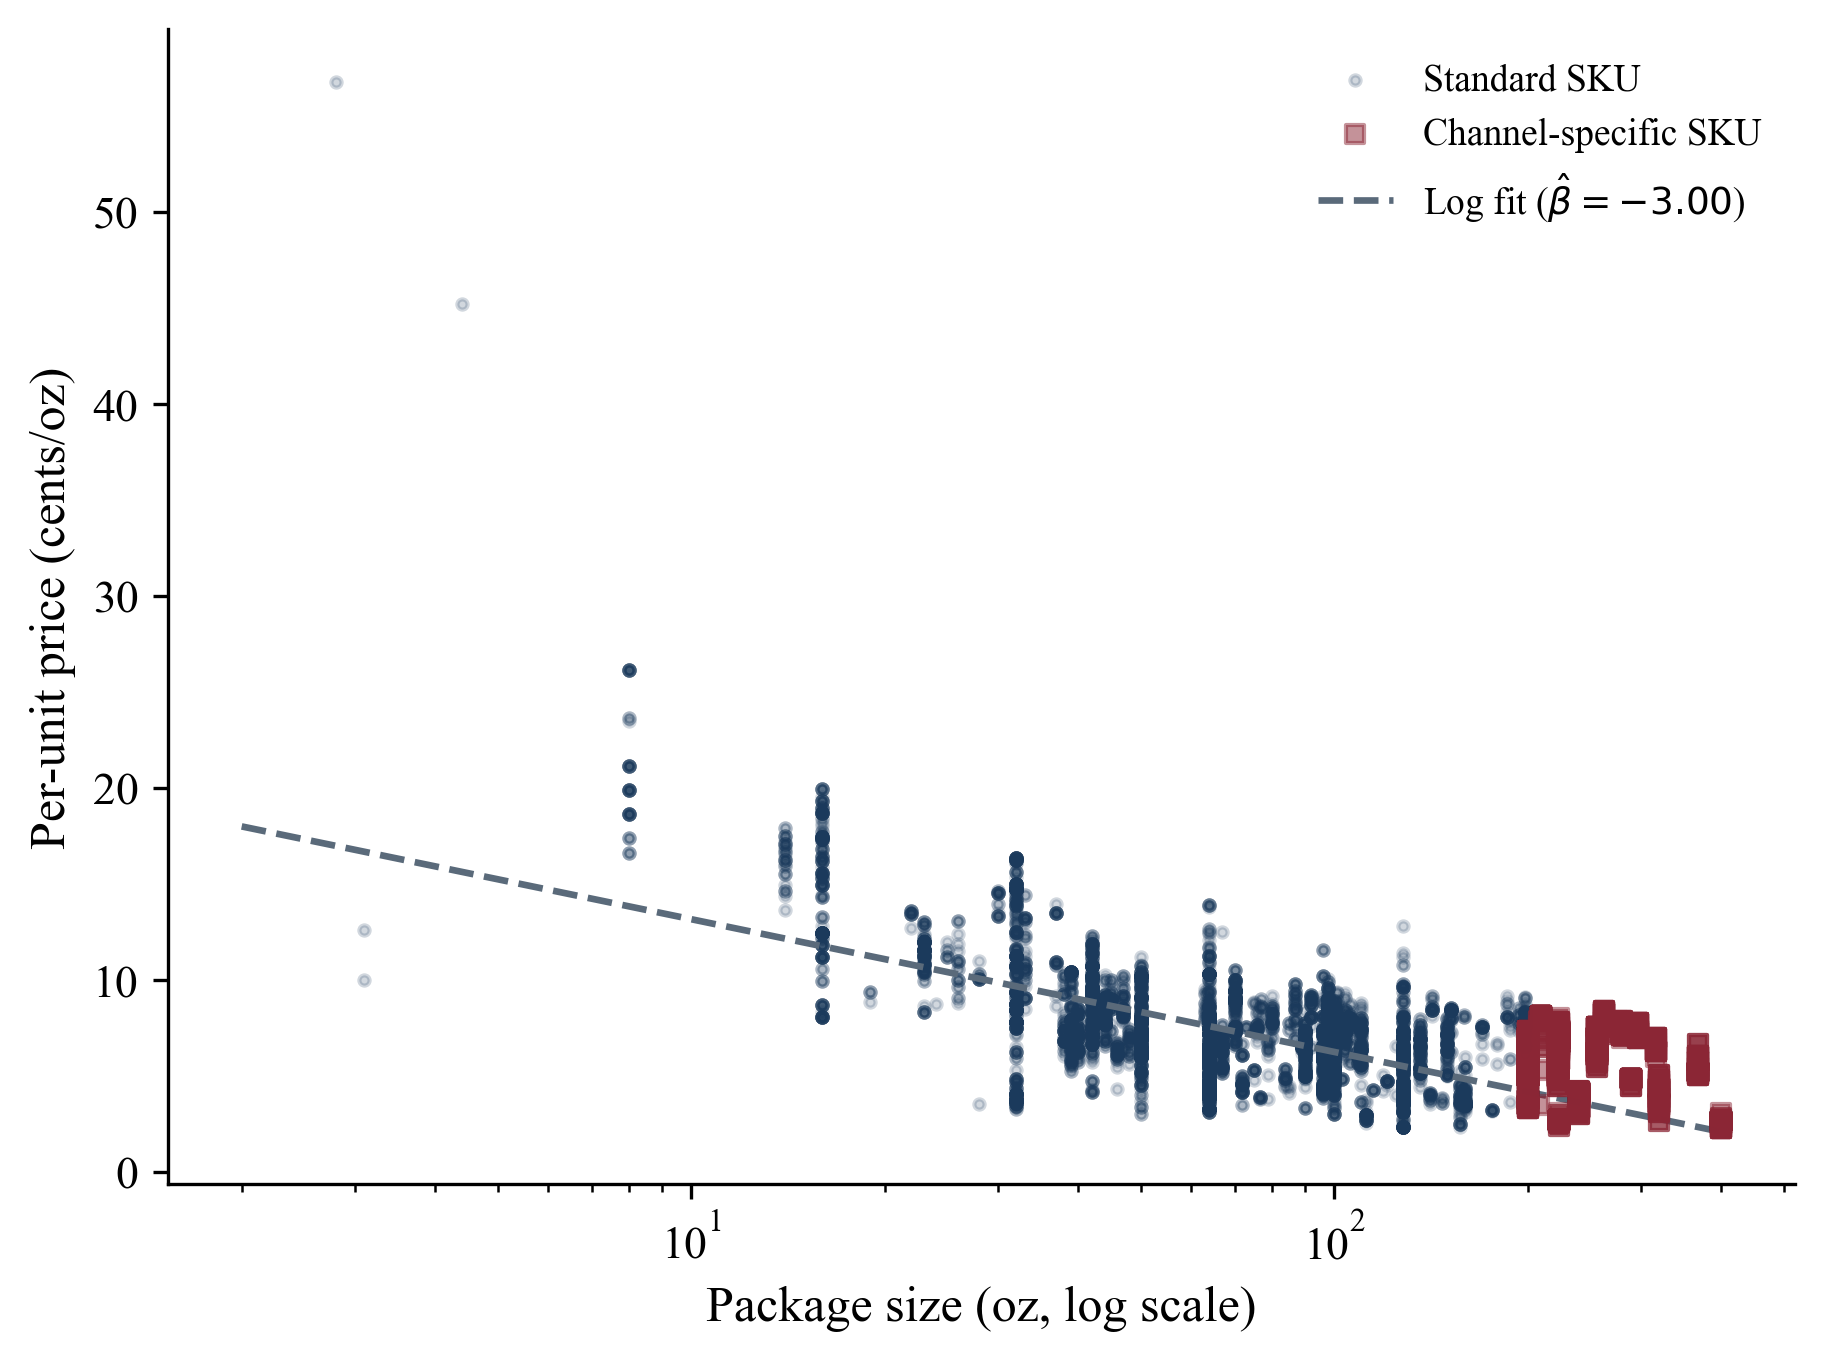
\includegraphics[width=0.82\textwidth]{fig3_scatter_channel.png}
\caption{Package size and per-unit price, distinguishing standard SKUs (circles) from large-format SKUs (squares, defined as the top 5\% of package sizes; proxy for bulk-oriented formats). The dashed line shows the overall log-linear fit. \textit{Source:} Author's calculations from Dominick's scanner data.}
\label{fig:scatter_channel}
\end{figure}

Figure~\ref{fig:boxplot_store} displays boxplots of per-unit price for the twelve Dominick's stores with the most observations, ordered by median.
There is visible variation across stores: median per-unit prices range from approximately 6.4 to 7.4~\textcent/oz.
This cross-store dispersion within a \textit{single retail chain} is consistent with a mixture of zone-pricing policy, local competitive conditions, and demand differences. The Dominick's Data Manual states that the chain priced products using 16 zones that effectively collapsed into four price tiers, with regular prices intended to be uniform within zones.\footnote{Dominick's Data Manual, University of Chicago Booth School of Business, Dominick's Finer Foods dataset documentation, local PDF consulted March 2026.}

\begin{figure}[H]
\centering
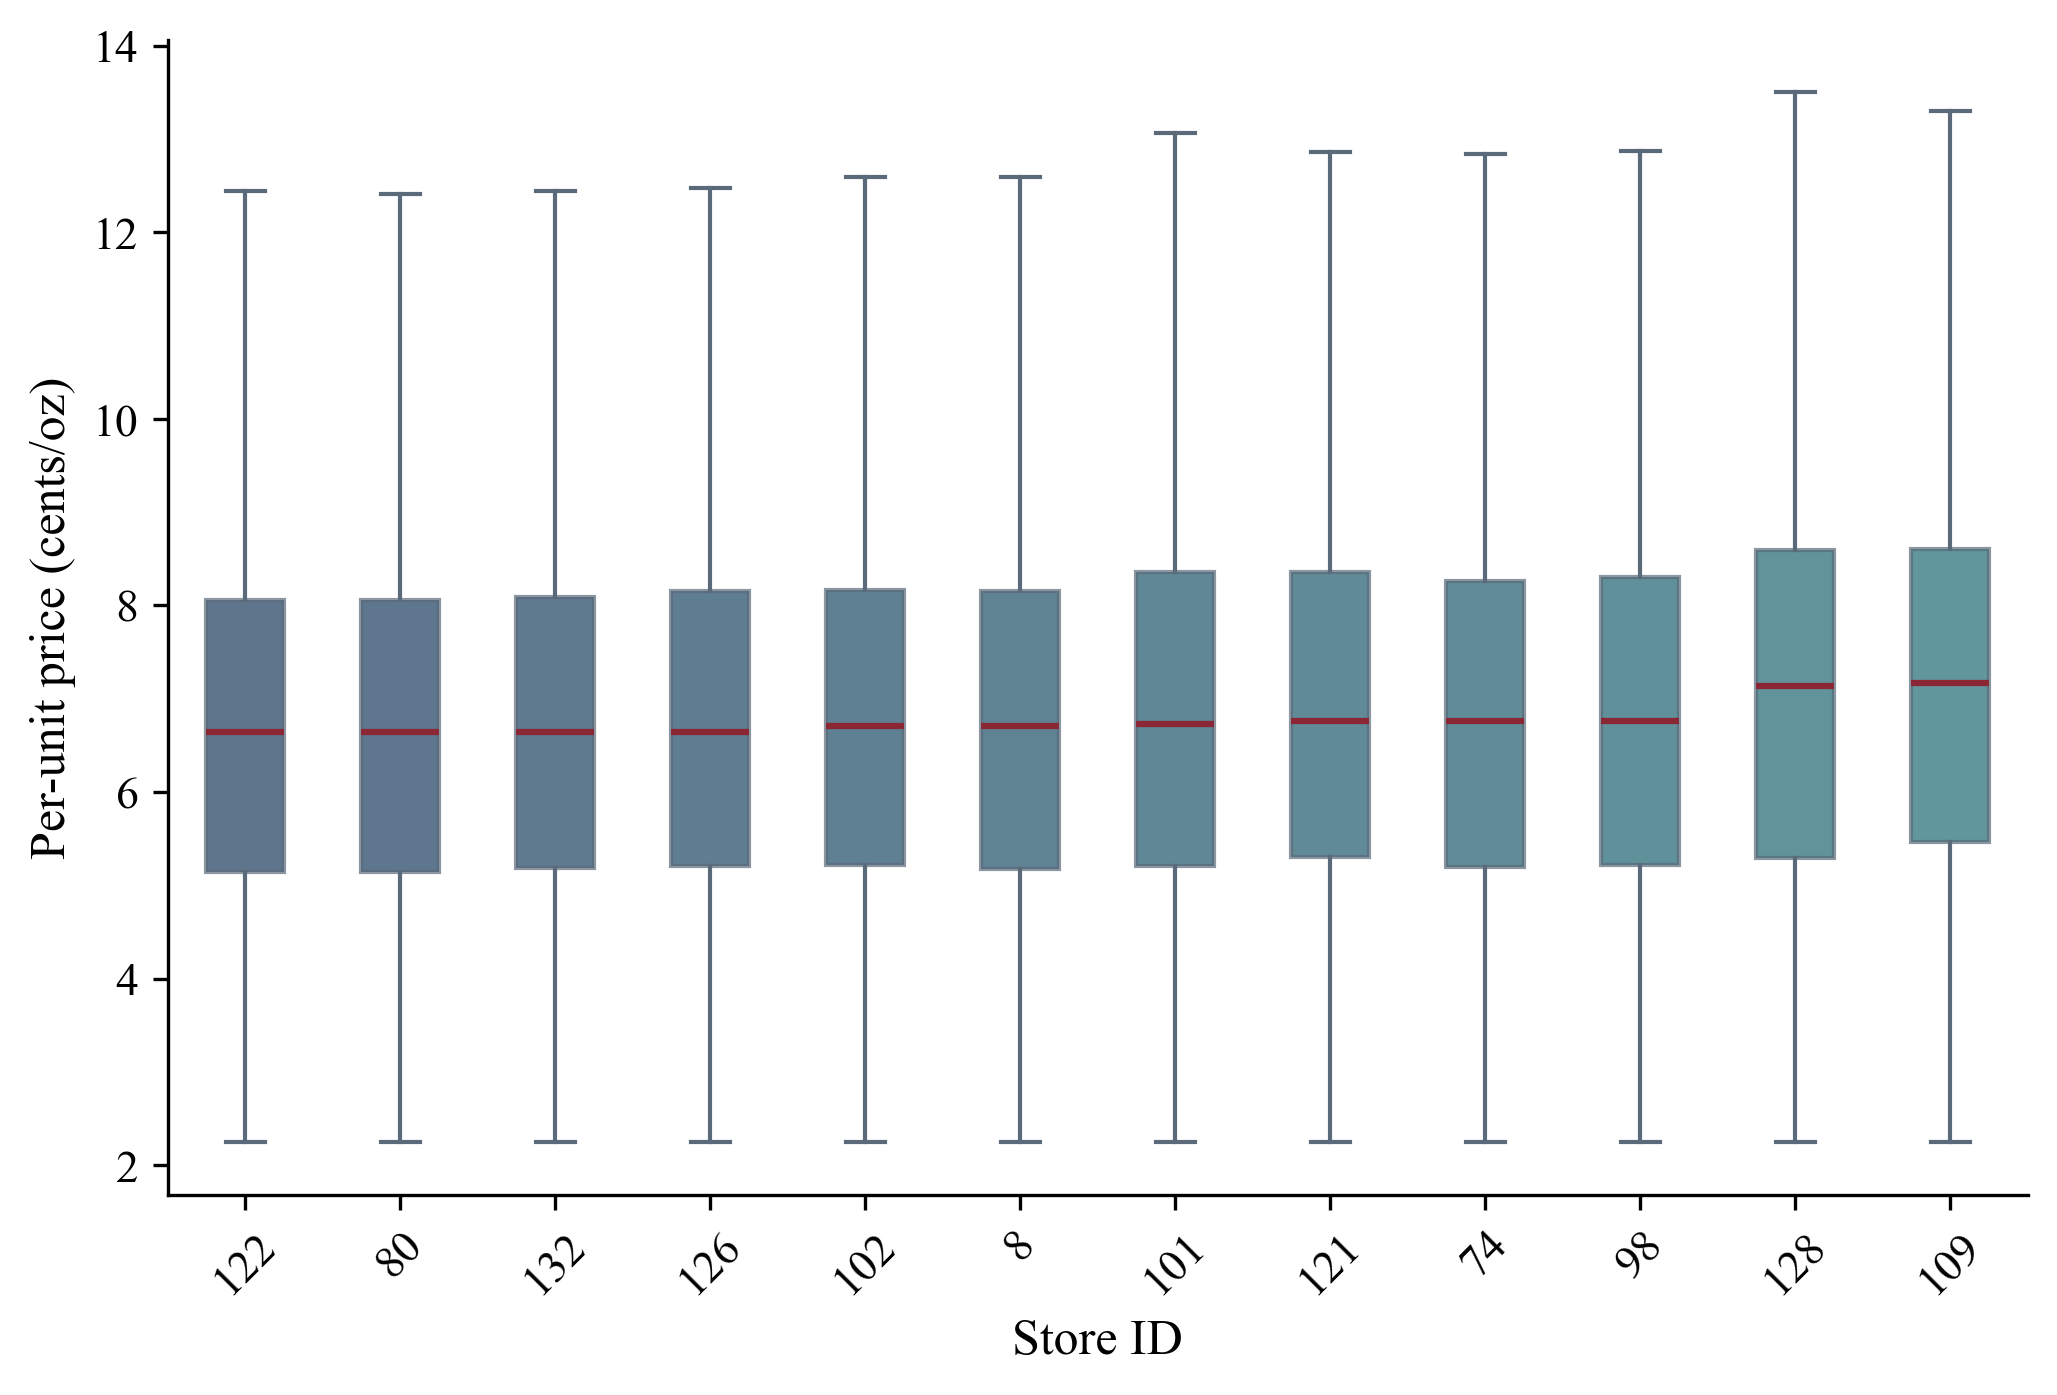
\includegraphics[width=0.82\textwidth]{fig7_ppu_by_store.png}
\caption{Per-unit price distribution by store (twelve highest-volume Dominick's stores, ordered by median). Outliers suppressed for clarity. \textit{Source:} Author's calculations from Dominick's scanner data.}
\label{fig:boxplot_store}
\end{figure}

Figure~\ref{fig:dist} shows the overall distribution of per-unit prices.
The distribution is right-skewed, with a long upper tail reflecting small-package, high-per-unit-price products.
The mean (7.2~\textcent/oz) exceeds the median (6.9~\textcent/oz). This is consistent with a mass of large, low-per-unit-price packages and a thinner tail of small, high-per-unit-price items.

\begin{figure}[H]
\centering
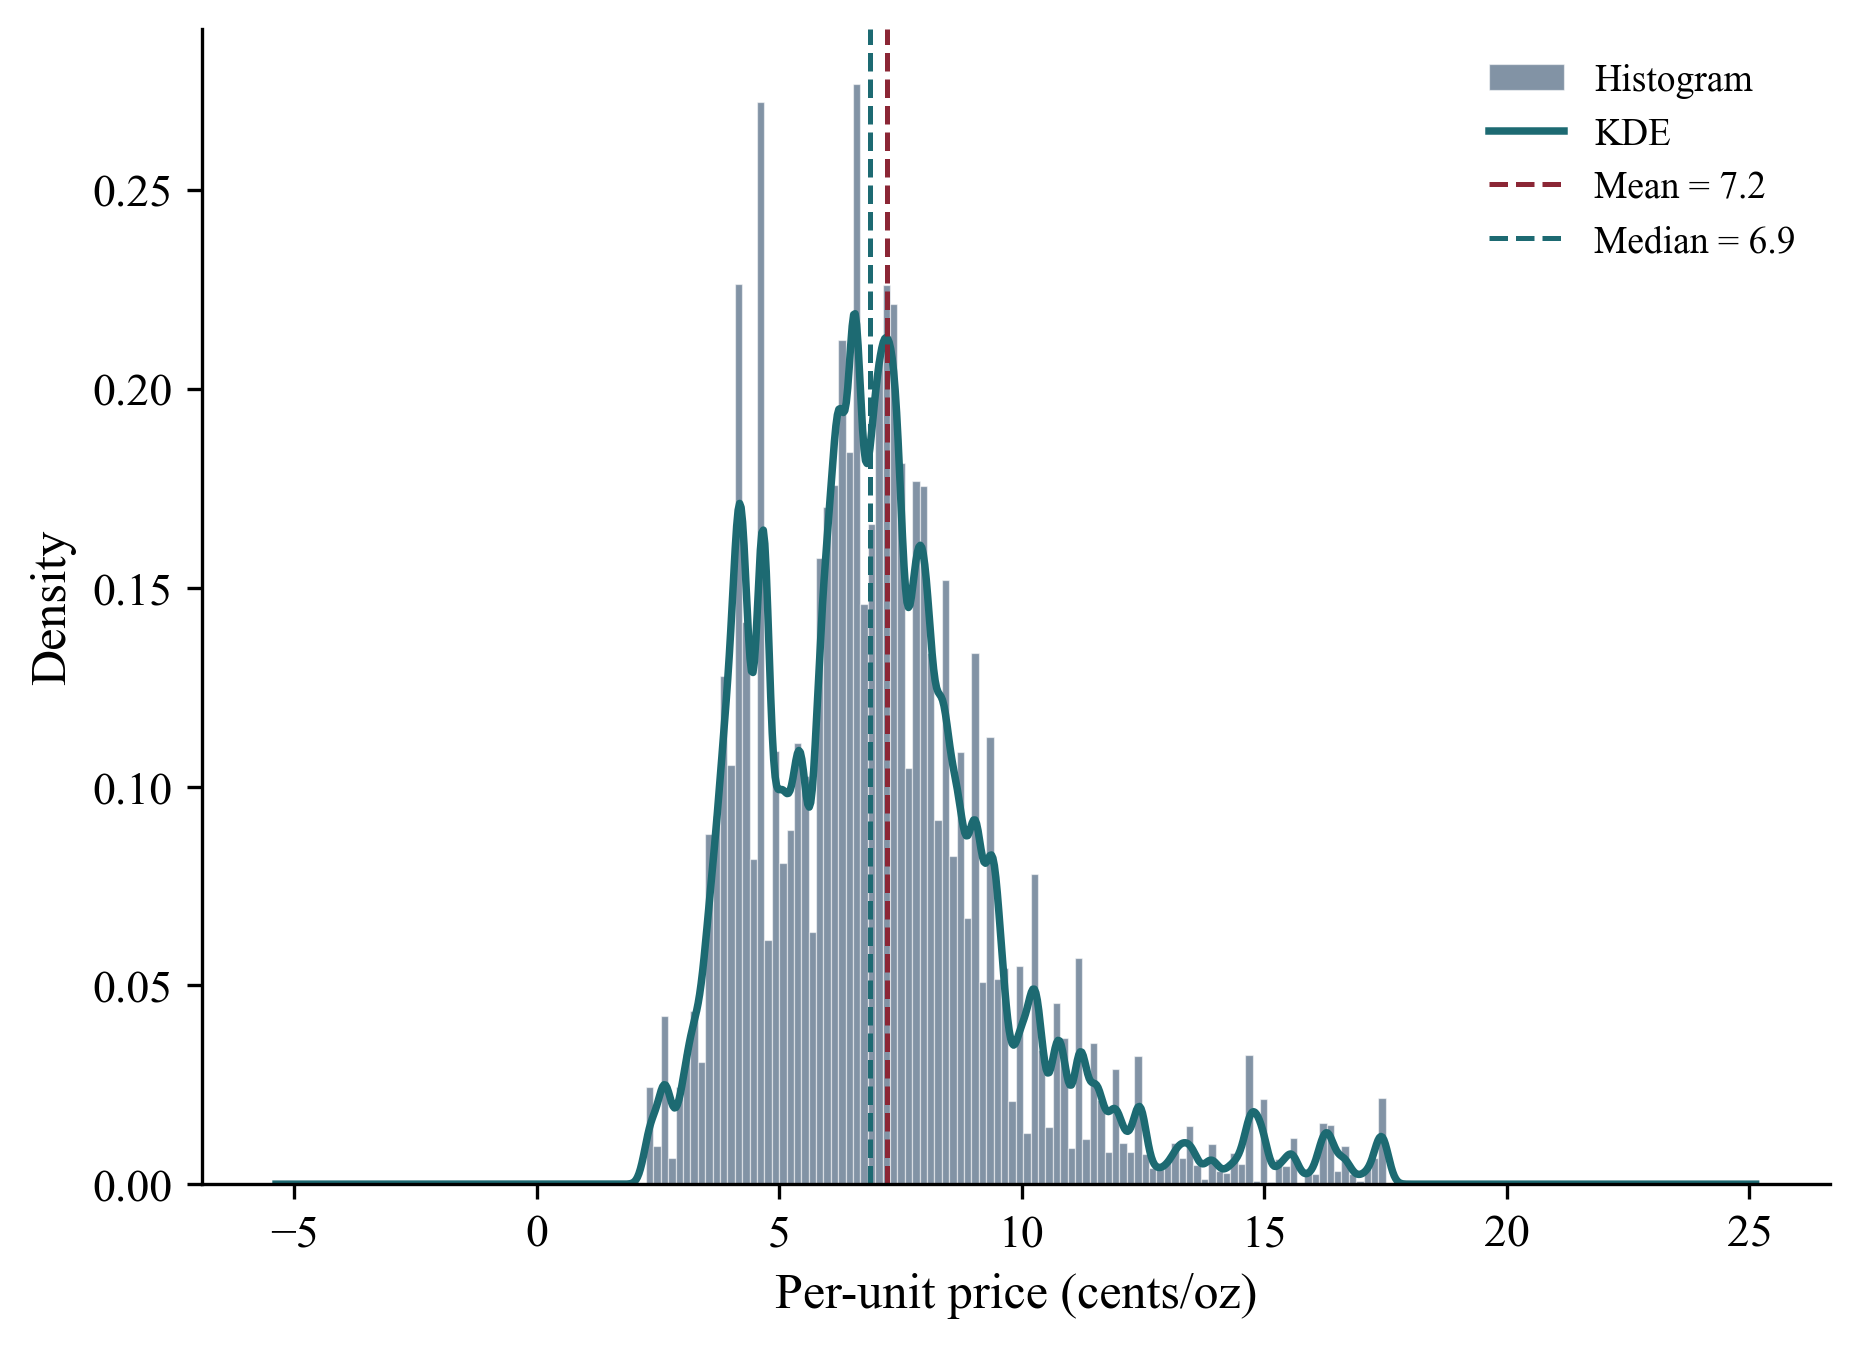
\includegraphics[width=0.82\textwidth]{fig8_ppu_distribution.png}
\caption{Distribution of per-unit prices across all store-week-UPC observations. Vertical lines mark the mean and median. \textit{Source:} Author's calculations from Dominick's scanner data.}
\label{fig:dist}
\end{figure}

\subsection{Regression specification and results}

The baseline regression estimates the size--price relationship:
\begin{equation}\label{eq:baseline}
\text{ppu}_{ijt} = \alpha + \beta\,\ln(\text{Size}_i) + \varepsilon_{ijt}. \tag{Baseline}
\end{equation}
Extensions add store fixed effects ($\gamma_j$), brand fixed effects ($\delta_b$), and a sale indicator:
\begin{equation}\label{eq:full}
\text{ppu}_{ijt} = \alpha + \beta\,\ln(\text{Size}_i) + \gamma_j + \delta_b + \phi\,\mathbf{1}[\text{Sale}_{ijt}] + \varepsilon_{ijt}. \tag{Full}
\end{equation}
All specifications report standard errors clustered by UPC to account for within-product correlation across stores and weeks.

Table~\ref{tab:regression} presents the results.
In the baseline specification~(1), $\hat{\beta} = -3.003$ (SE~$= 0.369$, $p < 0.001$) and $R^2 = 0.382$.
A one-log-point increase in package size (approximately a 2.7-fold increase) is associated with a 3.0~\textcent/oz decrease in per-unit price.
This large, precisely estimated coefficient shows that the size--price schedule is steeply declining. It is consistent with the quantity-discount logic of nonlinear pricing and with the model's prediction that size differentiation enables effective price discrimination.

Adding store fixed effects in specification~(2) leaves $\hat{\beta}$ essentially unchanged ($-3.007$) but yields a statistically significant improvement. A joint $F$-test on the 92 store dummies gives $F = 15.04$ ($p < 0.001$).
Per-unit prices differ systematically across stores even after controlling for product size.
This within-chain variation mirrors the cross-retailer heterogeneity in the theoretical model, where different downstream demand conditions motivate different effective wholesale prices.

Introducing brand fixed effects in specification~(3) raises $R^2$ from 0.385 to 0.470, a substantial increase.
The coefficient on log size attenuates slightly to $-2.820$. This indicates that part of the size--price gradient in the baseline reflects brand composition: premium brands cluster at certain sizes.
The remaining within-brand size gradient is large and highly significant. This is consistent with size-based pricing operating above and beyond brand effects.

The full model~(4) adds the sale indicator. It enters with a coefficient of $-0.606$ (SE~$= 0.079$, $p < 0.001$): promotional sales reduce per-unit prices by about 0.6~\textcent/oz on average.
The coefficient on log size is robust at $-2.800$.

\begin{table}[htbp]
\centering
\caption{Per-Unit Price Regressions: Dominick's Laundry Detergent}
\label{tab:regression}
\small
\begin{tabular}{lcccc}
\toprule
 & (1) & (2) & (3) & (4) \\
\midrule
$\ln(\text{Size})$ & $-3.003^{***}$ & $-3.007^{***}$ & $-2.820^{***}$ & $-2.800^{***}$ \\
 & $(0.369)$ & $(0.369)$ & $(0.366)$ & $(0.367)$ \\
[4pt]
Sale indicator &  &  &  & $-0.606^{***}$ \\
 &  &  &  & $(0.079)$ \\
[4pt]
Constant & $20.069^{***}$ & $20.405^{***}$ & $17.582^{***}$ & $17.613^{***}$ \\
 & $(1.656)$ & $(1.663)$ & $(1.623)$ & $(1.624)$ \\
\midrule
Store FE & No & Yes & Yes & Yes \\
Brand FE & No & No & Yes & Yes \\
\midrule
$R^2$ & 0.382 & 0.385 & 0.470 & 0.474 \\
Adj.\ $R^2$ & 0.382 & 0.385 & 0.470 & 0.474 \\
$N$ & 3,240,409 & 3,240,409 & 3,240,409 & 3,240,409 \\
\bottomrule
\end{tabular}

\medskip\par\noindent\footnotesize
\textit{Notes:} Dependent variable is per-unit price in cents per ounce. Standard errors clustered by UPC in parentheses. $^{***}\,p<0.01$, $^{**}\,p<0.05$, $^{*}\,p<0.10$. Store FE: 93 store dummies. Brand FE: 23 brand dummies.
\end{table}


\subsection{Robustness: alternative standard-error estimators}

Table~\ref{tab:robustness} re-estimates the full model under two alternative clustering schemes. The point estimates on $\ln(\text{Size})$ and the sale indicator are identical across all three columns, since clustering affects only the covariance estimator. Under store-level clustering (93 clusters), the standard errors are smaller than under UPC-level clustering (566 clusters). The very small standard error under store-level clustering reflects the fact that $\ln(\text{Size})$ varies at the UPC level rather than the store level; store-level clusters contain little identifying variation for this regressor. UPC-level clustering is therefore the more appropriate default, as supported by the two-way estimate. Under two-way clustering by UPC and store using the Cameron, Gelbach, and Miller (2011) formula, the standard errors are close to those from UPC-only clustering, supporting the conclusion that UPC-level dependence is the dominant source of within-sample correlation. All main coefficients remain significant at the 1-percent level across all three specifications.

% generated by robustness_table.py
\begin{table}[H]
\centering
\caption{Robustness Checks: Alternative Clustering Schemes (Full Model)}
\label{tab:robustness}
\begin{tabular}{lccc}
\toprule
 & (1) & (2) & (3) \\
 & UPC Clustered & Store Clustered & Two-Way Clustered \\
 & & & (UPC $\times$ Store) \\
\midrule
$\ln(\text{Size})$ & -2.800*** & -2.800*** & -2.800*** \\
 & (0.367) & (0.012) & (0.365) \\[4pt]
Sale indicator & -0.606*** & -0.606*** & -0.606*** \\
 & (0.079) & (0.015) & (0.080) \\[4pt]
\midrule
Store FE    & \checkmark & \checkmark & \checkmark \\
Brand FE    & \checkmark & \checkmark & \checkmark \\
$R^{2}$     & 0.474 & 0.474 & 0.474 \\
$N$         & \multicolumn{3}{c}{3,240,409} \\
\bottomrule
\multicolumn{4}{p{0.88\textwidth}}{\footnotesize \textit{Notes:}
Dependent variable: per-unit price (cents/oz). All three columns use
the same OLS regression with store and brand fixed effects; only the
covariance estimator differs. Cluster-robust standard errors in
parentheses. Column~(3) applies the Cameron, Gelbach, and Miller
(2011) two-way formula:
$\hat{V}_{\text{two-way}} =
 \hat{V}_{\text{UPC}} + \hat{V}_{\text{Store}}
 - \hat{V}_{\text{UPC}\times\text{Store}}$.
Point estimates are identical across columns.
$^{***}p<0.01$, $^{**}p<0.05$, $^{*}p<0.10$.}
\end{tabular}
\end{table}


\subsection{Within-brand regressions}

A natural objection to the size--price gradient is that it may reflect brand composition or package economics rather than deliberate price discrimination. To address this, Table~\ref{tab:within_brand} re-estimates the size--price regression separately for Tide, All, and Purex---three brands with substantial size variation in the Dominick's data.

Within each brand, larger packages carry significantly lower per-unit prices. The gradient is steepest for Purex ($\hat{\beta} = -3.13$, $p < 0.001$) and shallower for Tide ($\hat{\beta} = -0.74$, $p < 0.001$). These within-brand estimates rule out the possibility that the pooled gradient in Table~\ref{tab:regression} is merely picking up across-brand quality or formulation differences. The size--price schedule operates \textit{within} a single brand's product line, consistent with the model's prediction that manufacturers use size differentiation to segment consumers.

\begin{table}[htbp]
\centering
\caption{Within-Brand Size--Price Gradient}
\label{tab:within_brand}
\small
\begin{tabular}{lccc}
\toprule
 & Tide & All & Purex \\
\midrule
$\ln(\text{Size})$ & $-0.740^{***}$ & $-1.223^{***}$ & $-3.129^{***}$ \\
 & $(0.178)$ & $(0.401)$ & $(0.817)$ \\
[4pt]
Sale indicator & $-0.808^{***}$ & $-0.186$ & $-0.425^{*}$ \\
 & $(0.077)$ & $(0.130)$ & $(0.255)$ \\
\midrule
Store FE & Yes & Yes & Yes \\
\midrule
$R^2$ & 0.231 & 0.209 & 0.492 \\
Adj.\ $R^2$ & 0.230 & 0.209 & 0.492 \\
$N$ & 564,067 & 237,357 & 104,329 \\
UPCs & 78 & 51 & 22 \\
\bottomrule
\end{tabular}

\medskip\par\noindent\footnotesize
\textit{Notes:} Dependent variable is per-unit price in cents per ounce. Each column restricts the sample to a single brand. Standard errors clustered by UPC in parentheses. $^{***}\,p<0.01$, $^{**}\,p<0.05$, $^{*}\,p<0.10$. All specifications include store fixed effects and a sale indicator.
\end{table}


\subsection{Placebo check: per-unit price vs.\ total shelf price}

As a further diagnostic, Table~\ref{tab:placebo} regresses both per-unit price and total shelf price on log package size, with the same controls as the full specification. The coefficient on log size is strongly negative for per-unit price ($-2.80$, $p < 0.001$) but strongly positive for total shelf price ($+3.89$, $p < 0.001$). Larger packages cost more in absolute terms but less per ounce. This confirms a standard quantity-discount schedule, not a mechanical artefact of the per-unit calculation, and is consistent with nonlinear pricing theory.

\begin{table}[htbp]
\centering
\caption{Placebo Check: Per-Unit Price vs.\ Total Shelf Price}
\label{tab:placebo}
\small
\begin{tabular}{lcc}
\toprule
 & (1) PPU (\textcent/oz) & (2) Shelf price (\$) \\
\midrule
$\ln(\text{Size})$ & $-2.800^{***}$ & $3.893^{***}$ \\
 & $(0.367)$ & $(0.303)$ \\
[4pt]
Sale indicator & $-0.606^{***}$ & $-0.662^{***}$ \\
 & $(0.079)$ & $(0.088)$ \\
\midrule
Store FE & Yes & Yes \\
Brand FE & Yes & Yes \\
\midrule
$R^2$ & 0.474 & 0.652 \\
Adj.\ $R^2$ & 0.474 & 0.652 \\
$N$ & 3,240,409 & 3,240,409 \\
\bottomrule
\end{tabular}

\medskip\par\noindent\footnotesize
\textit{Notes:} Column~(1) uses per-unit price (cents per ounce) as the dependent variable. Column~(2) uses total shelf price (dollars). The negative coefficient in column~(1) and the positive coefficient in column~(2) confirm that larger packages have lower per-unit prices but higher total prices, ruling out a mechanical coding artefact. Standard errors clustered by UPC in parentheses. $^{***}\,p<0.01$, $^{**}\,p<0.05$, $^{*}\,p<0.10$.
\end{table}


\subsection{Interpretation and limitations}

The empirical results document pricing patterns consistent with the model.
First, the steep negative coefficient on log size corresponds to the model's mechanism of size-based product differentiation. By offering the same underlying product in different package sizes, the manufacturer can implement a nonlinear pricing schedule that approximates third-degree price discrimination.
Larger packages extract less surplus per unit from bulk-buying, more price-elastic consumers. Smaller packages extract more from convenience-oriented, less elastic consumers.

Second, the significant store fixed effects correspond to the model's retailer-heterogeneity parameter ($b_1 \ne b_2$).
Even within a single chain, where wholesale contracts are presumably uniform, zone-pricing policy, local demand conditions, and competitive environments generate meaningful variation in per-unit prices across locations.
In the cross-chain setting of the model, this variation would be amplified by differences in retail format and by the legal freedom to charge different wholesale prices for differentiated variants.

Several limitations should be noted.
First, the Dominick's data cover a single retail chain. The analysis therefore captures \textit{within-chain} variation rather than the \textit{cross-chain} discrimination that is the primary concern of Robinson--Patman.
The within-chain patterns are suggestive of the underlying mechanisms, but they cannot directly identify wholesale price discrimination.
Second, wholesale prices are not observed.
The model predicts that size-based retail price variation arises from size-based wholesale price discrimination. Without wholesale cost data, the retail-level patterns are consistent with this channel but do not prove it.
Third, the analysis is descriptive.
The coefficient on log size reflects a correlation between size and per-unit price, not a causal effect.
Unobserved product attributes correlated with size could contribute to the gradient.
In particular, package size is a manufacturer's strategic choice, not a random product feature. Larger detergent bottles may contain more concentrated formula, independently justifying lower per-unit prices. The ounce-based normalisation used here may not fully equalize washing capacity across products: a 100~oz bottle of concentrated formula may deliver more loads per ounce than a 100~oz bottle of standard formula. A more rigorous comparison would use load-equivalent pricing, but load counts are not available in the Dominick's data. The brand fixed effects in specification~(3) address quality differences at the brand level. Within a brand, the same core formulation typically appears across multiple package sizes, so the residual within-brand size variation is more credibly driven by deliberate nonlinear pricing. Formally establishing a causal effect would require an instrument for package-size choices; candidate instruments include store-level shelf-space constraints or wholesale-distribution logistics that determine which sizes each location stocks.
Fourth, the Dominick's data do not observe wholesale contracts, retailer-specific manufacturer variants, or cross-chain product allocation. Accordingly, the empirical analysis does not directly test whether manufacturers used minor product modifications to evade Robinson--Patman constraints; it documents retail pricing patterns that are \textit{consistent with} such a mechanism. Directly testing the wholesale discrimination channel would require matched wholesale--retail price data spanning multiple retail chains and product variants.

Fifth, Table~\ref{tab:robustness} supports the conclusion that the main results are robust to alternative clustering by store and to two-way clustering by UPC and store via the Cameron, Gelbach, and Miller (2011) formula. Point estimates are unchanged; standard errors under the two-way scheme are close to the UPC-clustered baseline.

Despite these limitations, the descriptive patterns are consistent with the model and with the institutional accounts of how manufacturers use package-size differentiation to segment channels under Robinson--Patman.


% CASE STUDIES REVISITED
\section{Case Studies Revisited}\label{sec:cases}

\subsection{Detergent package variants}

Manufacturers of laundry detergents, including Procter~\&~Gamble (Tide), Lever Brothers (Wisk, All, Surf), and others, offer a wide range of package sizes.
The Dominick's data are consistent with this pattern: Tide alone appears in sizes from 50~oz to over 200~oz, with per-unit prices ranging from roughly 5 to 12~\textcent/oz.
In the model, large club-store packages correspond to variant $A$ (high base demand, more elastic consumers). Smaller supermarket bottles correspond to variant $B$ (higher per-unit price, less elastic consumers).
The empirical size coefficient of $-3.0$ quantifies the per-unit price gradient that this differentiation exploits.

Legal analyses of \textit{Woodman's v.\ Clorox} show how restricting large packages to club stores triggers Robinson--Patman scrutiny.
By maintaining distinct SKUs, the manufacturer can set different wholesale prices while arguing that the products are not of like grade and quality.

\subsection{Branded versus authorized generics}

Pharmaceutical companies sometimes market chemically identical active ingredients under both a premium brand and a lower-priced authorized generic.
The products differ in packaging, tablet appearance, and labeling, but they share the same therapeutic function.
In the model, branded and generic versions correspond to variants $A$ and $B$, with different demand intercepts and slopes.
The differentiation cost $k$ reflects packaging and marketing expenses. The Robinson--Patman defense rests on arguing that branded and generic versions are not of like grade and quality because of differences in presentation.

\subsection{Retailer-exclusive mattress models}

The U.S.\ mattress market features retailer-exclusive models differing in quilting patterns, fabric covers, and minor construction details. The core components are nearly identical.
These cosmetic modifications create SKUs unique to each retailer, raising consumer search costs and limiting price competition.
In the model, the differentiation cost $k$ may be nontrivial. But if retailer demand conditions differ enough, the gain from variant-based discrimination exceeds $k$.

\subsection{International textbook editions}

Textbook publishers sell lower-priced international editions in developing markets. These are printed on cheaper paper with soft covers and different ISBNs.
The editions contain substantially the same content as domestic hardcovers but are physically downgraded.
In the model, international editions are low-cost variants targeting a more elastic segment abroad. The physical differences support lower prices and also make arbitrage less attractive.


% WELFARE IMPLICATIONS
\section{Discussion and Welfare Implications}\label{sec:welfare}

The model and empirical findings suggest that minor product modifications function as powerful instruments for retailer-level third-degree price discrimination under Robinson--Patman constraints.
From the manufacturer's perspective, these strategies increase profit by allowing prices to better match downstream demand conditions.
From the standpoint of consumers and social welfare, the implications are more nuanced.

On the one hand, variant-based discrimination can expand output in price-sensitive segments by enabling lower prices where demand is more elastic.
The Dominick's data show that large-package detergents carry per-unit prices roughly half those of small packages. This suggests that size-based discrimination does bring lower effective prices to bulk-buying consumers.
On the other hand, increased segmentation sustains higher prices in less elastic segments, raising distributional concerns.

Classical analyses show that welfare relative to uniform pricing depends on whether total output increases and how surplus is redistributed.\footnote{Richard Schmalensee, ``Output and Welfare Implications of Monopolistic Third-Degree Price Discrimination,'' \textit{American Economic Review} 71, no.~1 (1981): 242--247; Varian, ``Price Discrimination,'' 601--605.}
Appendix~\ref{app:welfare} derives the output condition formally.
In the manufacturer--retailer setting, Robinson--Patman constraints add a further dimension: variant-based discrimination is a response to legal rules that may or may not align with consumer welfare.
If enforcement focuses narrowly on formal equality of wholesale prices for identical commodities, firms may invest excessively in superficial differentiation, leaving underlying market power intact.
Stricter enforcement might then prompt \textit{more} product modification rather than less discrimination.
Enforcement that accounts for both functional substitutability and consumer welfare could discourage purely cosmetic variants while permitting efficiency-enhancing discrimination.

The cross-channel price dispersion that motivates the model is illustrated by a calibrated simulation in Appendix~\ref{app:simulations} (Figure~\ref{fig:retailer_box}), which shows per-unit prices highest in the grocery channel and lowest in club stores, with a gap of approximately 5~\textcent/oz.
Similarly, Figure~\ref{fig:welfare} (also in Appendix~\ref{app:simulations}) decomposes welfare under uniform pricing and under two-price discrimination. The net welfare effect depends on total output, as formalized in Appendix~\ref{app:welfare}.


% CONCLUSION
\section{Conclusion}\label{sec:conclusion}

This paper develops and analyzes a mechanism by which manufacturers use minor product modifications to implement retailer-level third-degree price discrimination under Robinson--Patman constraints.
A linear-demand model with a common-wholesale-price constraint shows that low-cost differentiation into channel-specific variants restores segment-specific wholesale prices and strictly increases manufacturer profit when downstream demand slopes differ.
The model provides closed-form expressions for the threshold differentiation cost $\bar{k}$ and connects the pricing result to the standard Ramsey inverse-elasticity condition.

Empirical analysis of the Dominick's Finer Foods scanner dataset, covering 3.24~million observations across 566~laundry-detergent UPCs, 93~stores, and 396~weeks, documents two pricing patterns consistent with the mechanism.
Per-unit prices decline steeply with package size ($\hat{\beta} = -3.0$, $p < 0.001$).
Per-unit prices vary significantly across stores ($F = 15.04$, $p < 0.001$).
Brand fixed effects account for a material share of price variation ($\Delta R^2 \approx 0.09$). This indicates that brand-level product differentiation is an additional channel for surplus extraction.

The institutional and legal background, particularly FTC guidance and \textit{Woodman's Food Market v.\ Clorox}, illustrates how package size, packaging, and retailer-exclusive SKUs navigate the boundary of ``like grade and quality.''
Future work could extend the model to endogenous retailer pricing, exploit wholesale cost data to test the discrimination channel directly, or use proprietary multi-chain scanner data to quantify cross-retailer discrimination and its welfare effects.\footnote{Data availability: The Dominick's Finer Foods dataset used in this paper is publicly available at the James~M.\ Kilts Center for Marketing, University of Chicago Booth School of Business (\url{https://www.chicagobooth.edu/research/kilts/research-data/dominicks}). All analysis code is available from the authors upon request.}


% APPENDICES
\appendix

\section{Welfare Comparison}\label{app:welfare}

Under linear demand $Q_i = a_i - b_i p_i$, consumer surplus in segment $i$ at price $p_i$ is
\begin{equation}\label{eq:cs}
CS_i(p_i) = \frac{(a_i - b_i p_i)^2}{2b_i} = \frac{Q_i^2}{2b_i}.
\end{equation}
Producer surplus in segment $i$ is $(p_i - c)\,Q_i$ (or $(w_i - c - k)\,Q_i$ with differentiation costs).

Under uniform pricing with $w^*$, retail prices are $p_i^U = w^* + m_i$, and quantities are $Q_i^U = a_i - b_i p_i^U$.
Under discrimination, retail prices are $p_i^D = w_i^* + m_i$, and quantities are $Q_i^D = a_i - b_i p_i^D$.

Total welfare under each regime is
\begin{align}
W^U &= \sum_{i=1}^{2}\left[\frac{(Q_i^U)^2}{2b_i} + (p_i^U - c)\,Q_i^U\right], \label{eq:wu}\\[6pt]
W^D &= \sum_{i=1}^{2}\left[\frac{(Q_i^D)^2}{2b_i} + (p_i^D - c - k)\,Q_i^D\right]. \label{eq:wd}
\end{align}

The standard result for linear demands is that third-degree price discrimination increases total welfare if and only if total output increases:
\begin{equation}\label{eq:welfare_condition}
W^D \ge W^U \quad\Longleftrightarrow\quad \sum_{i} Q_i^D \ge \sum_{i} Q_i^U.
\end{equation}
Substituting the closed-form quantities,
\begin{equation}\label{eq:output_condition}
\sum_{i} Q_i^D - \sum_{i} Q_i^U = \sum_{i} b_i\,(p_i^U - p_i^D) = \sum_i b_i\,(w^* - w_i^*).
\end{equation}
When $k = 0$ and the demand intercepts are symmetric ($a_1 = a_2$, $m_1 = m_2$), discriminatory and uniform prices coincide only if $b_1 = b_2$. With $b_1 \ne b_2$, the output effect in~\eqref{eq:output_condition} can be positive, negative, or zero depending on the specific parameter values. This is consistent with the classical result that discrimination via product modification does not unambiguously raise or lower welfare (Schmalensee, 1981; Varian, 1989).

For simplicity, the welfare expressions in~\eqref{eq:wu} and~\eqref{eq:wd} are stated with $k$ present only in the producer-surplus term. When $k > 0$, there is an additional real social cost $k\sum_i Q_i^D$ of producing the differentiated variants. This must be subtracted from $W^D$, making the net welfare gain from discrimination smaller. The output condition in~\eqref{eq:welfare_condition} then becomes necessary but not sufficient for a welfare improvement; one additionally requires the output expansion to dominate the differentiation cost.

When discrimination opens a new segment (for example, a club-store format that would not stock the product at the uniform price), total output necessarily increases, and welfare is more likely to rise.

\section{Robustness: Asymmetric Markups}\label{app:robustness}

The baseline model assumes fixed downstream markups $m_i$.
Here we verify that the results are qualitatively unchanged when markups differ across retailers ($m_1 \ne m_2$), as would be expected when retail formats have different cost structures.

With asymmetric markups, the uniform-pricing optimum (equation~\ref{eq:wstar}) becomes
\[
w^* = \frac{(a_1 + a_2) - (b_1 m_1 + b_2 m_2) + c(b_1 + b_2)}{2(b_1 + b_2)},
\]
and the discriminatory optima (equation~\ref{eq:wi}) become
\[
w_i^* = \frac{a_i - b_i m_i + b_i(c+k)}{2b_i}.
\]
The profit gain $\Pi^D(0) - \Pi^U$ is now positive whenever
\[
w_1^* \ne w_2^* \quad\Longleftrightarrow\quad \frac{a_1 - b_1 m_1}{2b_1} \ne \frac{a_2 - b_2 m_2}{2b_2},
\]
which is generically satisfied when either $b_1 \ne b_2$ or $m_1 \ne m_2$ (or both).
In other words, asymmetric markups provide an \textit{additional} source of heterogeneity that makes the uniform price suboptimal and strengthens the case for product modification.
The threshold $\bar{k}$ and the comparative statics from Proposition~\ref{prop:threshold} carry through with the appropriate relabeling of parameters.


\section{Simulation Figures}\label{app:simulations}

Figure~\ref{fig:retailer_box} presents an illustrative simulation of cross-channel price differences, calibrated to the Dominick's data and documented retail margins across grocery, mass-merchant, and club-store formats. This figure is a simulation, not a direct measurement, since the Dominick's data cover one supermarket chain. It illustrates the order of magnitude of cross-channel dispersion that motivates the model.

\begin{figure}[H]
\centering
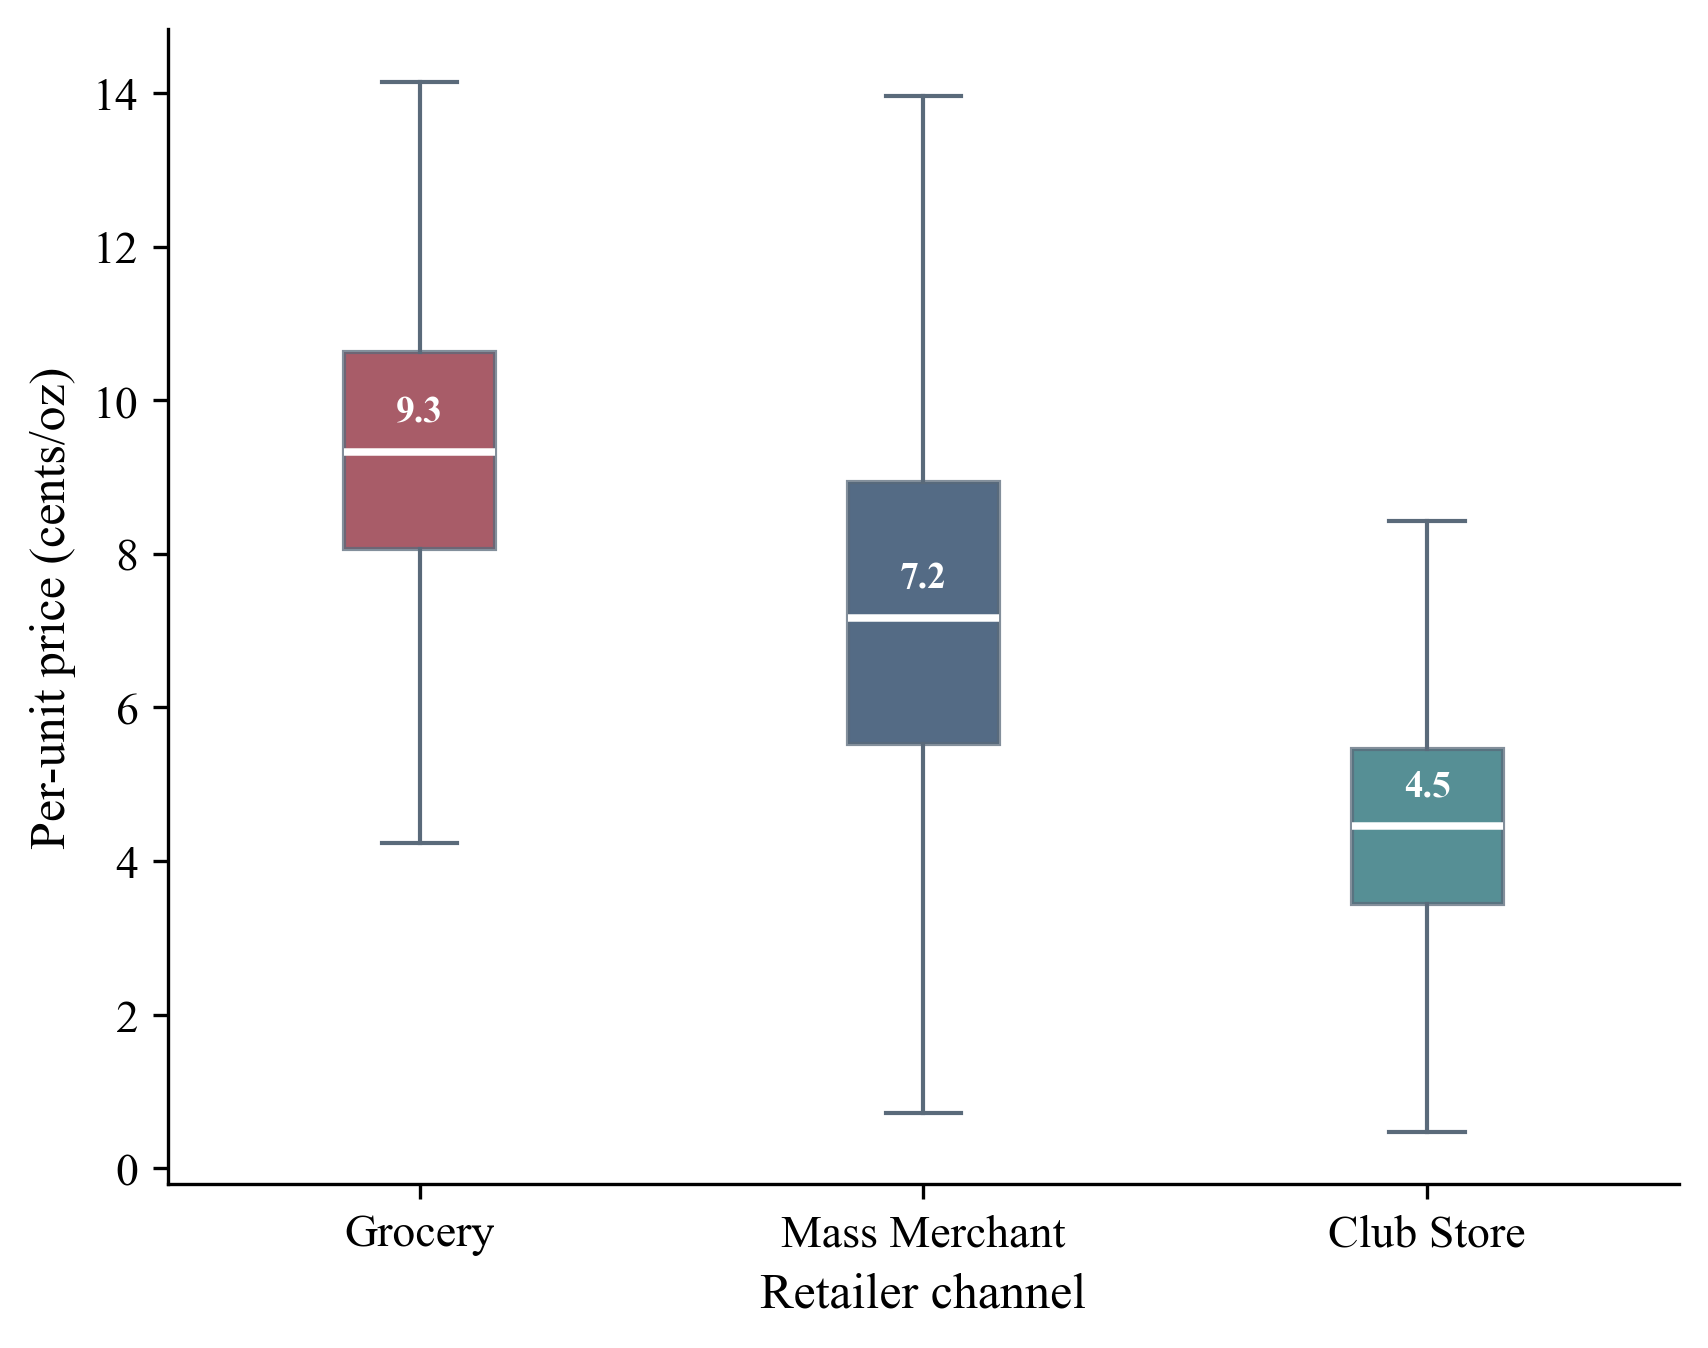
\includegraphics[width=0.72\textwidth]{fig2_retailer_boxplot.png}
\caption{\textit{Illustrative simulation.} Per-unit price distribution by retailer channel, calibrated to Dominick's data and documented retail margins for grocery, mass-merchant, and club-store formats. This figure is not a direct empirical measurement but illustrates the cross-channel price dispersion that motivates the model's heterogeneous-retailer setup. \textit{Source:} Author's calibration.}
\label{fig:retailer_box}
\end{figure}

Figure~\ref{fig:welfare} illustrates the welfare decomposition under uniform pricing and under two-price discrimination for two demand segments. Under discrimination, the deadweight-loss triangle shrinks in the elastic segment (served at a lower price) but may expand in the inelastic segment.

\begin{figure}[H]
\centering
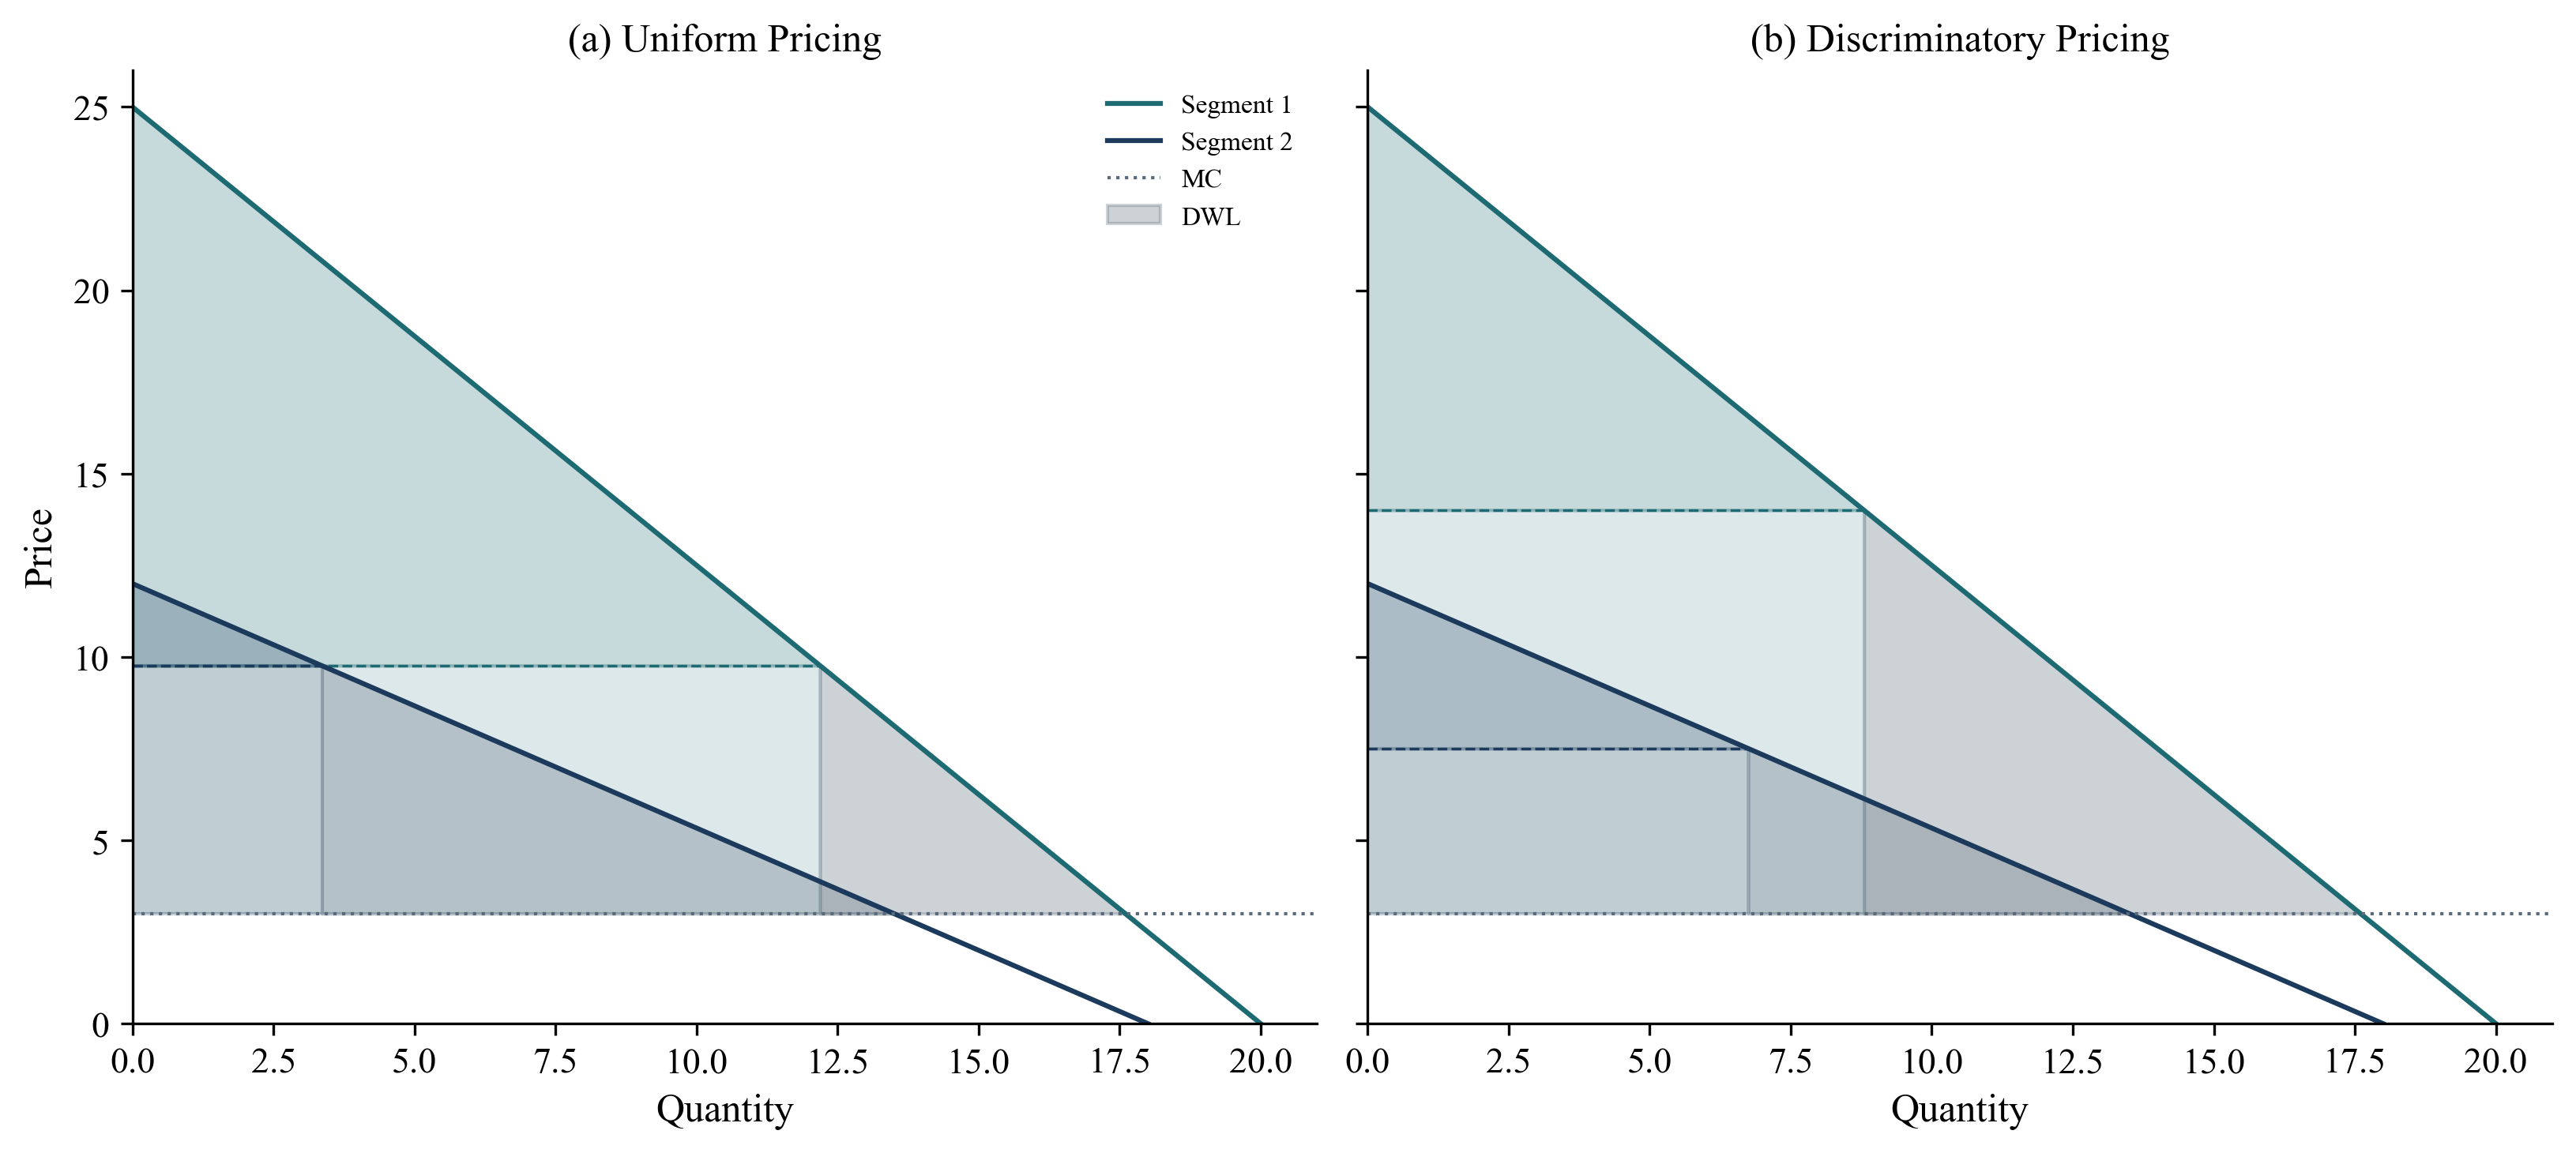
\includegraphics[width=0.95\textwidth]{fig5_welfare.png}
\caption{Welfare decomposition under (a) uniform pricing and (b) discriminatory pricing. Grey triangles represent deadweight loss. Consumer surplus and producer surplus areas shift across the two regimes. \textit{Source:} Author's calculations based on model parameters.}
\label{fig:welfare}
\end{figure}

% ACKNOWLEDGEMENTS
\section*{Acknowledgements}

The authors thank the James~M.\ Kilts Center for Marketing at the University of Chicago Booth School of Business for providing the Dominick's Finer Foods scanner dataset. The authors declare no conflicts of interest and received no external funding for this research.

\subsection*{AI Disclosure}
Portions of this paper were drafted, revised, and typeset with assistance from large-language-model tools (GitHub Copilot / Claude, OpenAI ChatGPT). These tools were used for code generation (Python data-cleaning and regression scripts), \LaTeX\ formatting, literature-search suggestions, and prose editing. All substantive analytical decisions---model specification, variable construction, interpretation of results, and legal analysis---were made by the authors. The authors take full responsibility for the accuracy and integrity of the final manuscript.

% REFERENCES
\newpage
\begin{thebibliography}{99}

\bibitem{FTC_RPA}
Federal Trade Commission.
``Price Discrimination: Robinson-Patman Violations.''
\url{https://www.ftc.gov/advice-guidance/competition-guidance/guide-antitrust-laws/price-discrimination-robinson-patman-violations}. Accessed March 2026.

\bibitem{Crowell2015}
Crowell \& Moring LLP.
``Do Different Size Packages Violate the Robinson Patman Act?''
Client Alert, March 2015.
\url{https://www.crowell.com/en/insights/client-alerts/do-different-size-packages-violate-the-robinson-patman-act}.
Accessed March 2026.

\bibitem{McGuireWoods2015}
McGuireWoods LLP.
``June Antitrust Bulletin.''
Client Alert, June 2015.
\url{https://www.mcguirewoods.com/client-resources/alerts/2015/6/june-antitrust-bulletin/}.
Accessed March 2026.

\bibitem{Woodmans2016}
\textit{Woodman's Food Market, Inc.\ v.\ Clorox Co.}, No.\ 15-3001 (7th Cir.\ 2016).
\url{https://law.justia.com/cases/federal/appellate-courts/ca7/15-3001/15-3001-2016-08-12.html}.
Accessed March 2026.

\bibitem{CrowellWoodmans2016}
Crowell \& Moring LLP.
``Woodman's v.\ Clorox: Does Size Matter? Not Always Under the Robinson-Patman Act.''
Client Alert, 2016.
\url{https://www.crowell.com/en/insights/client-alerts/woodman-s-v-clorox-does-size-matter-not-always-under-the-robinson-patman-act}.
Accessed March 2026.

\bibitem{Pigou1920}
Pigou, A.~C.
\textit{The Economics of Welfare}.
London: Macmillan, 1920.

\bibitem{Varian1989}
Varian, Hal~R.
``Price Discrimination.''
In \textit{Handbook of Industrial Organization}, vol.~1, edited by R.~Schmalensee and R.~Willig, 597--654.
Amsterdam: North-Holland, 1989.

\bibitem{KobayashiMuris2026}
Kobayashi, Bruce~H., and Timothy~J. Muris.
``Stop Making Sense: Reviving the Robinson-Patman Act and the Economics of Intermediate Price Discrimination.''
George Mason University / Competitive Enterprise Institute, February 2026.
\url{https://papers.ssrn.com/sol3/papers.cfm?abstract_id=6299819}.
Accessed March 2026.

\bibitem{Schmalensee1981}
Schmalensee, Richard.
``Output and Welfare Implications of Monopolistic Third-Degree Price Discrimination.''
\textit{American Economic Review} 71, no.~1 (1981): 242--247.

\bibitem{INET2018}
Institute for New Economic Thinking.
``Chicago School Economists Got it Wrong: Strong Antitrust Policy Boosts the Economy.''
2018.
\url{https://www.ineteconomics.org/perspectives/blog/chicago-school-economists-got-it-wrong-strong-antitrust-policy-boosts-the-economy}.
Accessed March 2026.

\bibitem{ITIF2024}
Information Technology and Innovation Foundation.
``No, Reviving the Robinson-Patman Act Will Not Lead to More Competition.''
November 2024.
\url{https://itif.org/publications/2024/11/25/reviving-robinson-patman-act-will-not-lead-to-more-competition-better-economy/}.
Accessed March 2026.

\bibitem{Winston2023}
Winston \& Strawn LLP.
``Price Discrimination Claims Under the Resurging Robinson-Patman Act.''
\textit{Competition Corner}, 2023.
\url{https://www.winston.com/en/blogs-and-podcasts/competition-corner/price-discrimination-claims-under-the-resurging-robinson-patman-act}.
Accessed March 2026.

\bibitem{Wilson1993}
Wilson, Robert~B.
\textit{Nonlinear Pricing}.
Oxford: Oxford University Press, 1993.

\bibitem{AdamsYellen1976}
Adams, W.~J., and J.~L. Yellen.
``Commodity Bundling and the Burden of Monopoly.''
\textit{Quarterly Journal of Economics} 90, no.~3 (1976): 475--498.

\bibitem{CBSWinners}
Ross, Thomas W.
``Winners and Losers under the Robinson-Patman Act.''
Copenhagen Business School Working Paper No.~30.
\url{https://ideas.repec.org/p/zbw/cbscwp/30.html}.
Accessed March 2026.

\bibitem{Dominicks}
Dominick's Finer Foods Dataset.
James~M.\ Kilts Center for Marketing, University of Chicago Booth School of Business.
\url{https://www.chicagobooth.edu/research/kilts/research-data/dominicks}.
Accessed March 2026.

\bibitem{DominicksManual}
Dominick's Data Manual.
University of Chicago Booth School of Business, Dominick's Finer Foods dataset documentation.
Local PDF consulted March 2026.

\bibitem{Yonezawa2020}
Yonezawa, Koichi, Miguel~I.\ G\'{o}mez, and Timothy~J.\ Richards.
``The Robinson--Patman Act and Vertical Relationships.''
\textit{American Journal of Agricultural Economics} 102, no.~1 (2020): 329--352.
\url{https://doi.org/10.1093/ajae/aaz049}.
Accessed March 2026.

\bibitem{KhanJain2005}
Khan, Romana~J., and Dipak~C.\ Jain.
``An Empirical Analysis of Price Discrimination Mechanisms and Retailer Profitability.''
\textit{Journal of Marketing Research} 42, no.~4 (2005): 516--524.

\end{thebibliography}

\end{document}
